\documentclass[letterpaper, 10pt, conference]{ieeeconf}
\usepackage{times}


\IEEEoverridecommandlockouts
\overrideIEEEmargins

\let\proof\relax
\let\endproof\relax

\usepackage{amsmath, amssymb}

\usepackage{url}

\usepackage[pdftex]{graphicx}

\usepackage{float}

\usepackage{relsize}

\usepackage{algorithm}

\usepackage{fancyvrb}

\usepackage[noend]{algorithmic}

\usepackage{subfiles}

\usepackage{titlecaps}

\usepackage{fancyhdr}

\usepackage{amsthm}

\renewcommand{\thefootnote}{\fnsymbol{footnote}}

\renewcommand{\algorithmicrequire}{\textbf{Input:}}
\renewcommand{\algorithmicensure}{\textbf{Output:}}

\newcommand{\tab}[1]{\hspace{.2\textwidth}\rlap{#1}}
\newcommand{\itab}[1]{\hspace{0em}\rlap{#1}}


\renewcommand{\thefootnote}{\fnsymbol{footnote}}
\newcommand{\Acronym}[1]{\ensuremath{{{\texttt{#1}}}}}
\newcommand{\Symbol}[1]{\ensuremath{\mathcal{#1}}}
\newcommand{\Function}[1]{\ensuremath{{ \textsc{#1}}}}
\newcommand{\Constant}[1]{\ensuremath{{\texttt{#1}}}}
\newcommand{\Var}[1]{\ensuremath{{{\textsl{#1}}}}}
\newcommand{\False}{\Constant{false}}
\newcommand{\True}{\Constant{true}}
\newcommand{\Null}{\Constant{null}}

\newcommand{\dif}{\ensuremath{{\mathrm{d}}}}

\newcommand{\Name}{\Acronym{Dodger}}

\newcommand{\Revision}[1]{\textcolor{red}{#1}}
\newcommand{\R}{\ensuremath{\mathbb{R}}}
\newcommand{\Traj}{\ensuremath{\zeta}}
\newcommand{\Tree}{\Symbol{T}}
\newcommand{\pair}[1]{\ensuremath{\langle#1\rangle}}

\newcommand{\argmin}[1]{\underset{#1}{\operatorname{arg}\,\operatorname{min}}\;}
\newcommand{\argmax}[1]{\underset{#1}{\operatorname{arg}\,\operatorname{max}}\;}

\newcommand{\mychange}[1]{\textcolor{red}{#1}}

\newtheorem{theorem}{Theorem}

\newtheorem{lemma}{Lemma}

\newtheorem{corollary}{Corollary}

%\setlength{\abovedisplayskip}{1pt}
%\setlength{\belowdisplayskip}{1pt}

\begin{document}

\title{Generating Safe Trajectories in Stochastic Dynamic Environments by
Leveraging Information about Obstacle Motion}


\author{Alex Wallar \and Erion Plaku \and Michael Weir
\thanks{A. Wallar and M. Weir are with the School of Computer Science,
  University of St Andrews, Fife KY16 9AJ, Scotland, UK. E. Plaku is with the
  Dept. of Electrical Engineering and Computer Science, Catholic
  University of America, Washington DC 20064 USA.
}}

\maketitle

\begin{abstract}

    In the domain of mobile robotics, the ability for a robot to navigate
    safely through an uncertain dynamic environment is a core component of
    autonomy.  In many situations, the motion of dynamic obstacles is
    predictable. This information can be used by a planner to generate safe,
    collision free paths to the goal. This paper develops a novel probabilistic
    representation of dynamic obstacles using their predicted trajectories that
    can account for an obstacle diverging from its prescribed path. This
    representation is used to add time dependent costs on the edges of a
    probabilistic roadmap (PRM). A graph search algorithm is presented that can
    find safe paths through the PRM to guide a robot from its initial
    configuration to a goal configuration amidst stochastic dynamic obstacles.
    The developed planning approach is shown to outperform a potential fields
    planner for guiding a robot in multiple situations and for different
    notions safety.

\end{abstract}


\section{Introduction}

\label{chapter:introduction}

Path planning is a very important problem in robotics and computer science. It
is the problem of generating a path through an environment that if followed by
a robot, would move the robot from some initial configuration to a goal
configuration without coming into collision with any obstacles on the way. This
problem may seem easy for a human to solve, just walk around the obstacles and
get to the goal, but for a robot it can be extremely difficult. As humans, we
have amazing perception abilities and an unparalleled ability to assess the
risk we perceive and plan around it. These capabilities are not as developed in
artificial intelligence. Humans can walk around environments which are dynamic
and uncertain and (usually) reach wherever they are going without running into
moving obstacles or hitting walls. This is because as humans, we can determine
automatically where things are going to be in the future by looking at their
past locations and use this information to build safe, collision free paths to
our goals. Imagine you are driving a car and reach an intersection, you stop
because you see a car coming from the right. You have a choice to either move
forward crossing over the future path of the other car, or to wait for the car
to pass. By judging how far the car is away from you and how fast it is moving,
you can automatically determine whether or not it is safe to cross the road.
Likewise, imagine you are a waiter in a busy, hectic restaurant. You have to
bring an order to hungry customers. You are able to bring the customers the
food by predicting where other waiters and customers are going to be whilst you
move through environment in order to avoid spilling the food and sacrificing
your tip. Our brains do this planning and prediction automatically in order to
generate safe paths through stochastic dynamic environments. The aim of this
project is to use given information about the future motion of obstacles by an
external system in order to generate safer paths than state of the art planners
that have been designed for and operate in dynamic environments.

There has been outstanding progress by the robotics community to develop
algorithms that are able to plan the motion of a robot in order for it to reach
its goal. From this community, three different paradigms for path generation
and motion planning have emerged, geometric algorithms, reactive algorithms,
and sampling based approaches~\cite{choset, lavalle}. Geometric algorithms such
as the bug algorithm~\cite{weir} or visibility graph algorithm~\cite{vis}, use
the geometry of the environment to create exact geometric paths to the goal.
These algorithms almost always have no random component, and for a given
environment, will return the same path every time. The second paradigm for
motion planning, reactive algorithms, move the robot to the next best location
at the current time for a given sensing radius. These approaches are vastly
dominated by the use of potential fields in order to determine the direction
that a robot should move. The approaches use a combination of an attractive
potential function to guide the robot towards a goal and a repulsive potential
function that keeps the robot from coming into contact with obstacles. The
robot moves forward in time by determining the direction it should move that
would minimize the combined potentials. Sampling based approaches approximately
discretize the environment, also known as the search space, in order to
describe its connectivity by sampling plausible configurations and how to move
between them.  With the discretization, usually in the form of a graph or a
tree, paths to the goal are extracted using shortest path algorithms which seek
to minimize a given objective function. These approaches are becoming
exceedingly popular due to their running time and how they are able to scale
for high dimensional systems.

This project aims to utilize developments in motion planning, particularly
sampling based motion planning in order to move a robot safely from an initial
configuration to a goal configuration in a stochastic dynamic environment by
leveraging information about the trajectories of dynamic obstacles. By having
some idea about where the obstacles are going to move in the future, it is
possible to use sampling based techniques that can sample collision free and
low risk paths to the goal in space-time. The goal of this project is to create
algorithms that can provide low cost paths to the goal by utilizing the
information available about how the obstacles in an environment will move. This
work introduces a novel representation of dynamic obstacles and a novel
algorithm for searching the environment in space-time.  Proofs are also
provided that can guarantee the completeness of the search such that the
algorithms will always provide a path to the goal. This problem is important
because if robots are interacting with humans, the robot must move safely in
order not to come into contact with and hurt humans as well as minimize the
damage that can possibly occur to itself. Likewise, imagine a situation where a
robot is deployed to an environment for a long period of time. By generating
safe paths (i.e. paths that have an insignificant chance of colliding with an
obstacle), the robot can be deployed for longer periods of time without
maintenance, because it would be less likely that it would get damaged as a
result of a collision. A solution to this problem can provide safer paths for
the operating environment and the robot by leveraging information that can be
extracted about where obstacles are moving.  Likewise, this problem is
important because there exists systems that are able to predict the motions of
obstacles, however there is a lack of systems that use this knowledge to
generate safe paths.

This work is structured by first outlining the formal objectives for the
project, the definition of a dynamic obstacles and its probabilistic
representation, the algorithms developed using this representation to move the
robot to the goal, a description of the experimental setup, analysis of the
empirical results, and a discussion regarding the evaluation of the approach
and future work.

\section{Related Work}

\label{chapter:contextsurvey}

For years the planning community has been developing algorithms that allow
robots to navigate through environments to reach a goal. As research
progressed, so did the complexity of the environments that the robots needed to
move through. It started with static obstacles which remain stationary for the
entirety of the execution, then on to dynamic obstacles with stochastic motion,
to dynamic obstacles that have predictable paths that planners can exploit. For
the last situation, a number of planners implementing different techniques have
been created. Techniques include evolutionary computation on geometric
structures in space-time to generate paths, safe interval path planning,
sampling based space-time search using collision prediction, and probabilistic
methods. Note that this context survey only covers approaches that make use of
models of obstacle behaviour and discards approaches that purely react to
obstacle motion.

\subsection{Evolutionary Algorithms}

Wang et al.\ used a genetic algorithm~\cite{galletly1992overview} that would
generate a path around the static and dynamic obstacles~\cite{wang2007mobile}.
The obstacles were encoded by a set of vertices in a polygon. The chromosomes
used in the genetic algorithms represented the paths that the robot can take to
move to the goal where the path is comprised of the initial and goal points
along with obstacle vertices.  The path generated for the robot would cling to
the perimeters of obstacles, until the robot could move towards the goal
similar to the bug algorithm~\cite{weir}. The time at which the robot would
reach each node was also encoded into the path. Moving obstacles were
represented as static obstacles for a given time. Upon a sensed change in the
environment such as a dynamic obstacle veering off its prescribed trajectory,
the genetic algorithm was used to regenerate a collision free path.

Smierzchalski and Michalewicz have also used an evolutionary
approach~\cite{evosurvey} where the chromosome represents the spatio temporal
path in order to plan the movements of a ship in a harbour where the obstacles
are other ships in shipping lanes~\cite{smierzchalski2005path}. The higher the
evaluation for the chromosome (i.e.\ the path) the safer and shorter the path
is. Unlike the work done by Wang et al.\ the path can be comprised of any point
in the search space.  The obstacles were represented geometrically and the
dynamic obstacles were represented by their initial configuration and velocity.
Since the path represented in a spatio-temporal fashion, the genetic algorithm
is able to determine if a path will collide with a dynamic obstacle by deducing
where the dynamic obstacle will be at each time step along the path and
checking for a collision.  Replanning using the evolutionary algorithm was
implemented to account for obstacles deviating from their prescribed
trajectories.

Dunwei and Na used particle swarm optimization (PSO)~\cite{kennedy2010particle}
to generate local paths around dynamic obstacles that are represented by
trajectory bands~\cite{dunwei2011local}.  In order to account for the
stochasticity in the obstacle trajectories, a distance around each obstacle's
trajectory was used to describe how much the obstacle can deviate from it.
Using these bands, an objective function was created that represents the safety
of a generated path and PSO was used to generate a path that could minimize the
objective function.

\subsection{Safe Interval Path Planning}

Narayanan et al.\ and Phillips et al.\ have developed algorithms for generating
safe paths to guide a robot to a goal configuration by determining time
intervals for which it would be safe to travel through certain areas in the
search space and using a graph search algorithm to find a path to the goal that
only intersects safe time intervals~\cite{asipp, sipp}.  Safe time intervals
are determined by iterating through the trajectory of each obstacle and
updating a query structure that can be used to check whether a certain space
will be free for a given period of time. A lattice structure is used to
discretize the search space and an A* variant, Anytime Reparing A*
(ARA*)~\cite{likhachev2003ara} is used to search this lattice. This algorithm
relies on the robot waiting at certain locations for areas to become free of
obstacles before it is able move towards the goal.

\subsection{Sampling in Space-time}

Berg et al.\ have developed a sampling based approach that generates a
probabilistic roadmap of the same dimension as the configuration space of the
robot with time that takes into account static and dynamic obstacles.
\cite{van2006anytime}. A novel graph search technique similar to D*
Lite~\cite{koenig2002d} was implemented that can automatically repair the path
when new information about obstacle motion is available such that the robot
will not be led into a collision with an obstacle. Obstacles are represented by
elongated objects in space-time and their stochasticity is represented by their
size as the time away from the current time increases.

Hsu et al.\ have also created an algorithm that generates a probabilistic
roadmap in space-time where each node represents the configuration of the robot
and a time at which the robot would be at the
configuration~\cite{hsu2002randomized}. Using the probabilistic roadmap, a
shortest path algorithm is used to find the fastest route from the initial
configuration of the robot to the goal configuration. Obstacles are represented
in a similar fashion as the work done by Berg et al.~\cite{van2006anytime}
except there is no representation of stochasticity. The planner handles updated
information about the dynamic obstacles by updating the probabilistic roadmap
and researching the graph for a path to the goal.

\subsection{Probabilistic Methods}

Jensen et al.\ developed an algorithm that uses a probabilistic obstacle model
to represent and employs a gradient decent method to find a path to the
goal~\cite{jensen2003motion}. A gradient decent approach tries to minimize the
probability of the robot coming into collision with an obstacle along the path.
This method is general but assumes that the robot has a sensing radius and is
able to move in the direction that has the lowest probability of collision.
Likewise, the paper shows that the combined probability model for the obstacles
in the scene only has one global minima. The algorithm can also be adapted so
that there is a trade off between the probability of collision and the length
of the path.

Rodriguez et al.\ uses a dynamic probabilistic roadmap to find a global path to
the goal and local kinodynamic motion planning to evade dynamic
obstacles~\cite{rodriguez2007framework}. A self-repairing probabilistic roadmap
is generated that takes into account the location of static obstacles. Using
this roadmap, a global path to the goal is found using a graph search
technique. The global path represents a sequence of sub-goal regions and a
kinodynamic local planner using an approach similar to RRT~\cite{rrt}
determines the local path that moves the robot to each sub-goal region in
sequence. This approach allows obstacles which have been assumed to be
stationary to move or have uncertainty in their positions. The probabilistic
roadmap will automatically repair itself upon obtaining updated information
about the static obstacles such that no edge is in collision with an obstacle.

\subsection{Limitations of Related Work}

The main limitation of the developments described is that there is no solution
that uses the obstacles' known stochastic trajectories to build probabilistic
representations and use these representations to build complete low cost paths.
Some of the algorithms currently either assume that the planner only knows that
the obstacles will move randomly around a point~\cite{rodriguez2007framework}
or that the obstacles will move along a fixed
trajectory~\cite{hsu2002randomized}, and if they deviate, a new plan is
developed. Hsu et al.\ assumed perfect information about the obstacle
trajectories to build an initial path through the environment, and if the
information was incorrect or the obstacles deviate from their prescribed
trajectories, the planner develops a new route to the goal. Berg et al.\
increased the size of the dynamic obstacles in space time to account for random
motion, but to plan around them, represented the obstacles as static objects in
space-time thus not devising a cost metric for their motion. Likewise, the
approaches that used safe interval path planning~\cite{asipp, sipp}, did not
build probabilistic models of the obstacles, but instead determined intervals
at which it would be safe to travel through certain areas and is thus heavily
reliant on the robot waiting at certain locations. The evolutionary approaches
described were geometric and also did account for the stochasticity in the
known trajectories of the dynamic obstacles. The one approach that did create
probabilistic models of the dynamic obstacles~\cite{jensen2003motion} employed
a gradient decent method similar to that of potential fields that is described
in Sec.~\ref{sec:costpf} to be ineffective in certain situations and that a
sampling based approach is more complete. All of these approaches lack an
elegant, sampling based algorithm that can take into account the stochastic
trajectories of dynamic obstacles in order to rely less heavily on replanning,
and to make use of the available information from the environment. The approach
described in this work develops a formal representation dynamic obstacles that
is able to take into account their stochasticity and presents a novel sampling
based approach that is able to generate low cost paths that can lead a robot to
its goal.

\section{Planner Methodology}

\label{chapter:methodology}

As described briefly in Sec.~\ref{sec:finaldesign}, the final planner design
uses a probabilistic roadmap to capture the connectivity of the environment and
uses a novel variant of best first search to find a safe, low cost path to the
goal. This approach is called Dodger. This section describes the algorithm as
well as formalizes the definition of a dynamic obstacle and its associated cost
distribution and motion.

\subsection{Dynamic Obstacles}

As a major component of this work, dynamic obstacles need to be designed such
that one can describe their trajectories, initial configurations, and their
levels of uncertainty. This section introduces the definition of a dynamic
obstacle used throughout this work along with how one is represented to the
planner and its simulated \& predicted equations of motion. Specifically, the
formal definition of a dynamic obstacle will be introduced, a novel way of
representing obstacles using a cost distribution will be formalized, and their
predicted and simulated motion will be described.

\subsubsection{Definition}

\label{sec:def}

A dynamic obstacle is defined as a 5-tuple, $a = (I, \dot{\zeta},
\epsilon, \xi, T)$ where $I$ is the initial configuration of the obstacle,
$\dot{\zeta}$ is a function, $\dot{\zeta}: \mathbb{R}^+ \rightarrow
\mathbb{R}^2$, representing the velocity of the obstacle, $\epsilon$ is used to
define a random variable $\rho \sim \mathcal{U}(-\epsilon, \epsilon)$ that is
used to inject noise into an obstacle's trajectory shown in
Eq.~\ref{eq:obs_observed} where $\mathcal{U}$ is a uniform distribution, $\xi$
is the current configuration used for prediction, and $T$ is the time that the
obstacle was in configuration $\xi$.  The variables $\xi$ and $T$ are dynamic
variables and are updated throughout the execution of the algorithm and are
used to determine when it is appropriate for the algorithm replans and finds a
new path through the environment using more up to date information. This is
explained in Sec.~\ref{sec:design_planner}. The variables $\xi$ and $T$ are
initially set to $I$ and $0$ respectively. It is assumed that the robot has
access to this information about the dynamic obstacles and will use it to
safely move around them. Information such as the initial configuration and the
velocity equation for each dynamic obstacle are assumed to be determined by an
external system that is either using a machine learning technique to deduce
these properties by using information about where the dynamic obstacle has been
before or by an external planning system such as in a warehouse that is
commanding the velocities and configurations of these dynamic obstacles. This
is the same assumption as that made by Phillips et al~\cite{sipp} and Narayanan
et al~\cite{asipp}.

\subsubsection{Cost Distribution}

\label{sec:cost}

Unlike in the previous work, dynamic obstacles are represented by cost
distributions that resemble probability density functions. The difference being
is that these cost distributions do not have a unit integral. These cost
distributions are used to describe where the obstacle is going to be in within
a time interval and can be generated by a third party system, such as a motion
capture system. There is an assumption that for a given interval, $\mathcal{T}
= [t_0, t_m]$, the highest cost with the smallest uncertainty will be at $t =
t_0$ and the lowest cost with the highest uncertainty will be at $t = t_m$.
Under this assumption, the cost function models how the obstacle may diverge
from its current trajectory as time increases. With these assumptions, the cost
function, $P_a: \mathbb{R}^2 \times (\mathbb{R}^+)^2 \rightarrow
\mathbb{R}$, represents the cost surface for a given dynamic obstacle, $a$,
within a given time interval. Eq.~\ref{eq:singleprob} formally defines the cost
function for a single obstacle.

% Single agent PDF

\begin{equation}
    P_a(x, y, t_0, t_m) = \frac{1}{t_m} \cdot \int^{t_m}_{t_0}
    \mathcal{N}(\zeta_a(t), \alpha \cdot (t - t_0)^2 + \beta, x, y) \cdot
    (t_m - t + 1)^{\gamma} \,\mathrm{d}t
    \label{eq:singleprob}
\end{equation}

In Eq.~\ref{eq:singleprob}, $\mathcal{N}(\mu, \sigma^2, x, y)$ is the
evaluation of a 3D normal distribution centered at $(\mu_x, \mu_y)$ with a
variance of $\sigma^2$ at $(x, y)$ and $\alpha$, $\beta$, and $\gamma$ are
scaling constants such that $\alpha > 0$, $\beta > 0$, and $\gamma \geq 1$.
Fig.~\ref{fig:normal_3d} shows an example of $\mathcal{N}$. The normal
distribution works as a basis function to describe the possible trajectories of
the dynamic obstacle. This equation models how the uncertainty of obstacle
trajectory prediction increases over time by increasing the standard deviation
of the Gaussian distribution as the time increases.  Likewise, this function
multiplies the Gaussian distribution by a factor of $(t_m - t)^{\gamma}$ where
$\gamma \geq 1$ which gives higher costs to times closer to $t_0$.

\begin{figure}[h!]
    \centering
    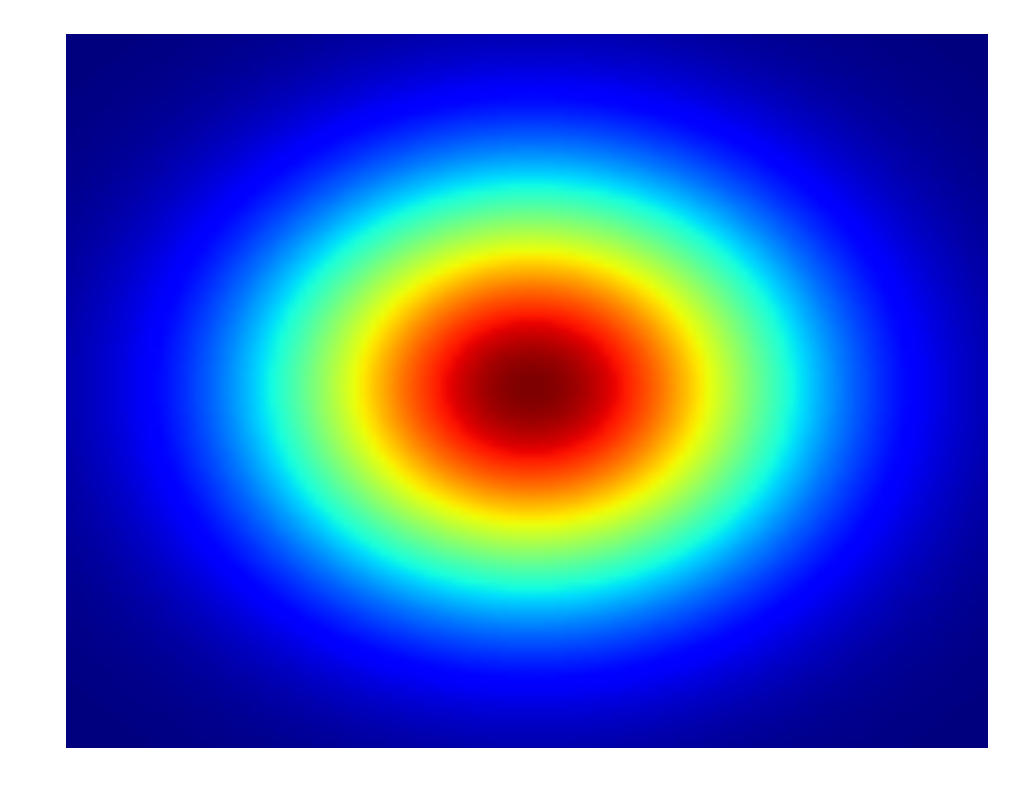
\includegraphics[width=0.60\linewidth]{figs/normal_3d}

    \caption{A plot depicting the three dimensional normal distribution
    $\mathcal{N}(\cdot)$ that is used as a basis function for the obstacle cost
distribution. The more red an area, the higher the cost. The more blue an area,
the lower the cost.}

    \label{fig:normal_3d}
\end{figure}

A cost function is also needed that can incorporate the cost distributions for
multiple dynamic obstacles within the environment. The cost function used in
this work, $P: \mathbb{R}^2 \times (\mathbb{R}^+)^2 \times \mathcal{A}
\rightarrow \mathbb{R}$ where $\mathcal{A}$ is the set of all possible sets of
dynamic obstacles, calculates the average cost at a point $(x, y)$ within a
given time interval for a given set of dynamic obstacles, $A$. This is shown
formally in Eq.~\ref{eq:prob}.

% Multiple agent PDF

\begin{equation}
    P(x, y, t_0, t_m, A) = \frac{\mathlarger{\sum_{a \in A} P_a(x, y, t_0,
    t_m)}}{|A|}
    \label{eq:prob}
\end{equation}

An example of how $P$ changes over time is shown in Fig.~\ref{fig:agent_cost}.
In that example, two dynamic obstacles are placed in the scene and given
sinusoidal velocities. In this example the time interval, $\delta t$, is kept
constant throughout the simulation, i.e. $t_m = t_0 + \delta t$, for all $t_0
\in [0, T - \delta t]$ where $T$ is the length of the simulation. Since the
velocity does not remain constant in the example, the cost distribution
elongates an shrinks based on the acceleration of the obstacle. For instance,
in the first and last images in Fig.~\ref{fig:agent_cost}, the cost is
contained to a small area due to the velocity equations of the obstacles being
at their minimum and in the fourth image, the cost is more spread out through
the environment because the velocity is at its maximum.

\begin{figure}[h!]

    \centering

    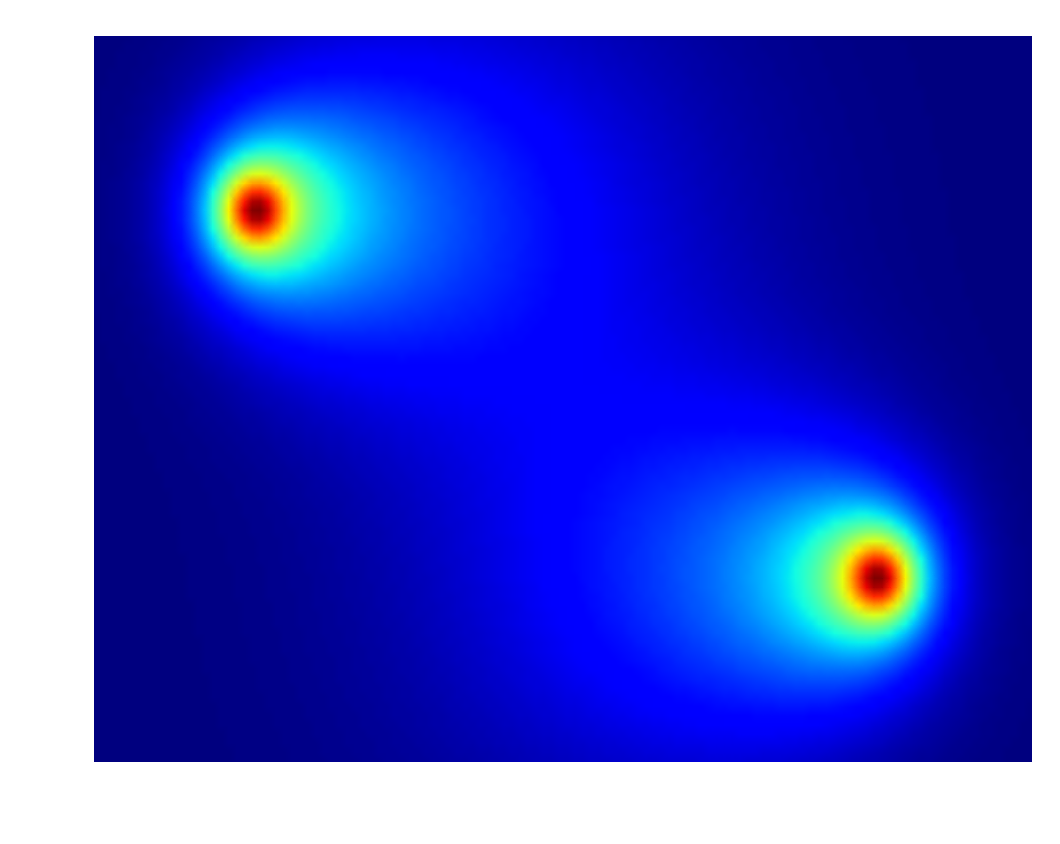
\includegraphics[width=0.24\linewidth]{figs/agent_1}
    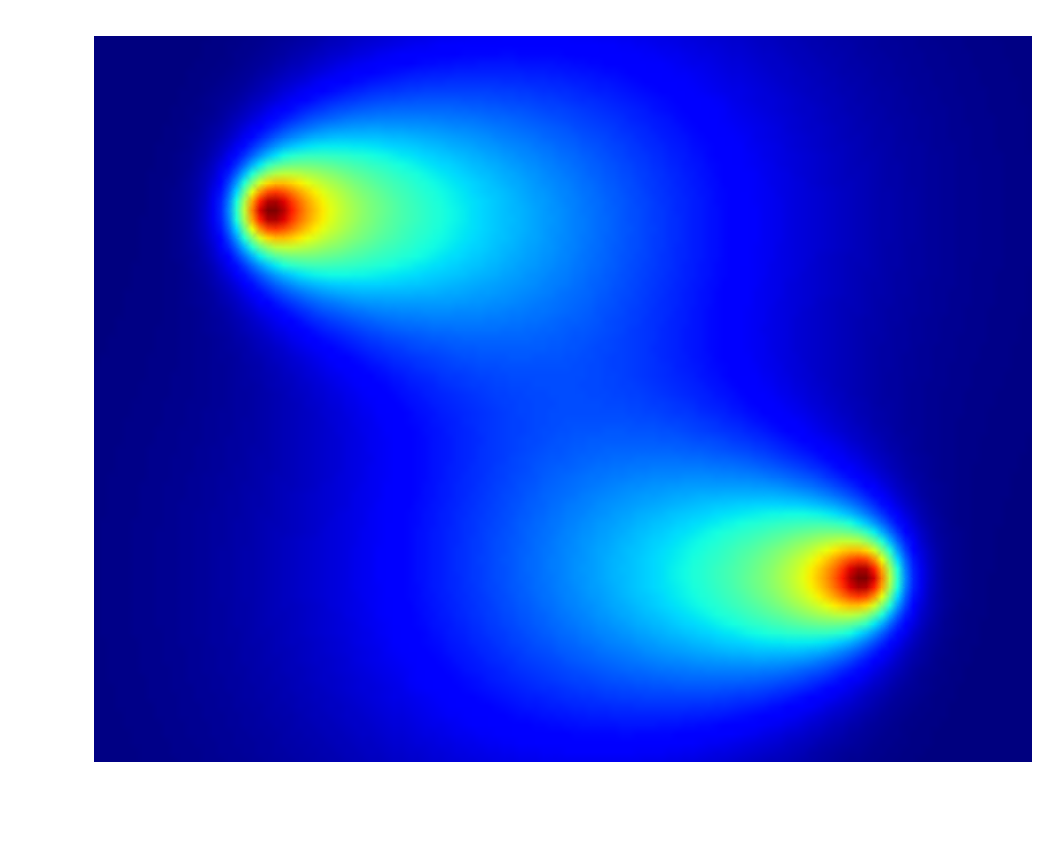
\includegraphics[width=0.24\linewidth]{figs/agent_2}
    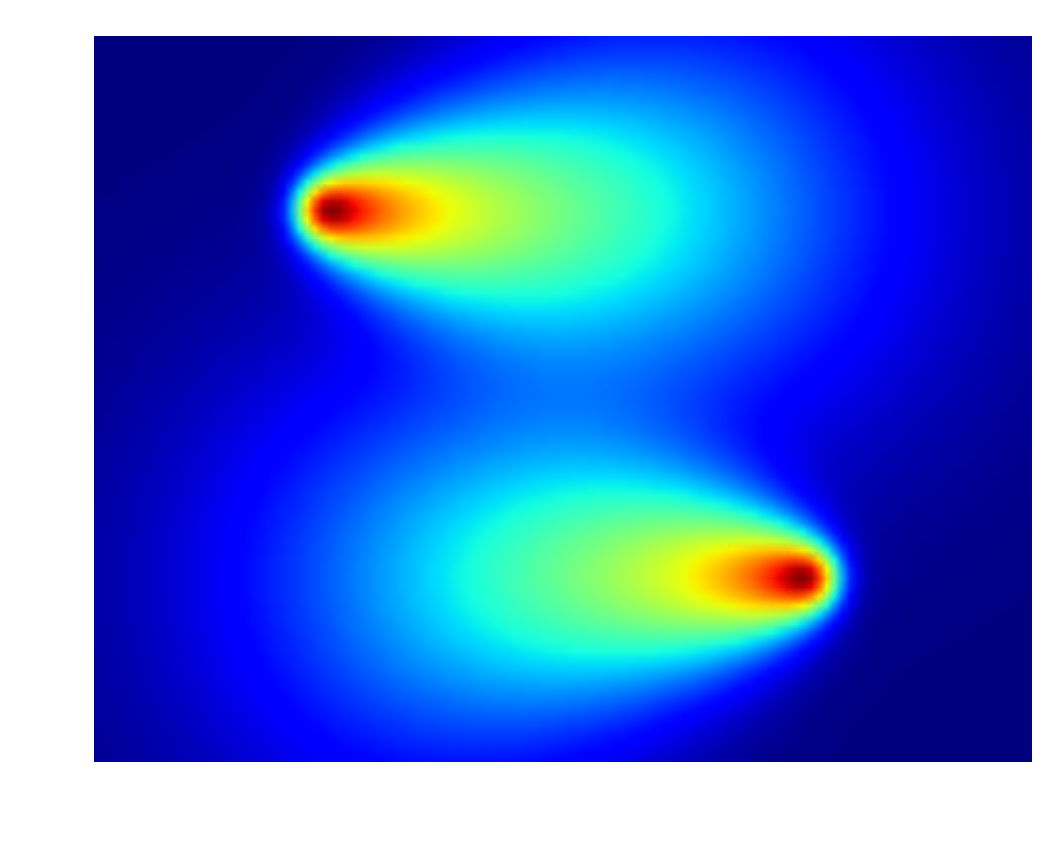
\includegraphics[width=0.24\linewidth]{figs/agent_3}
    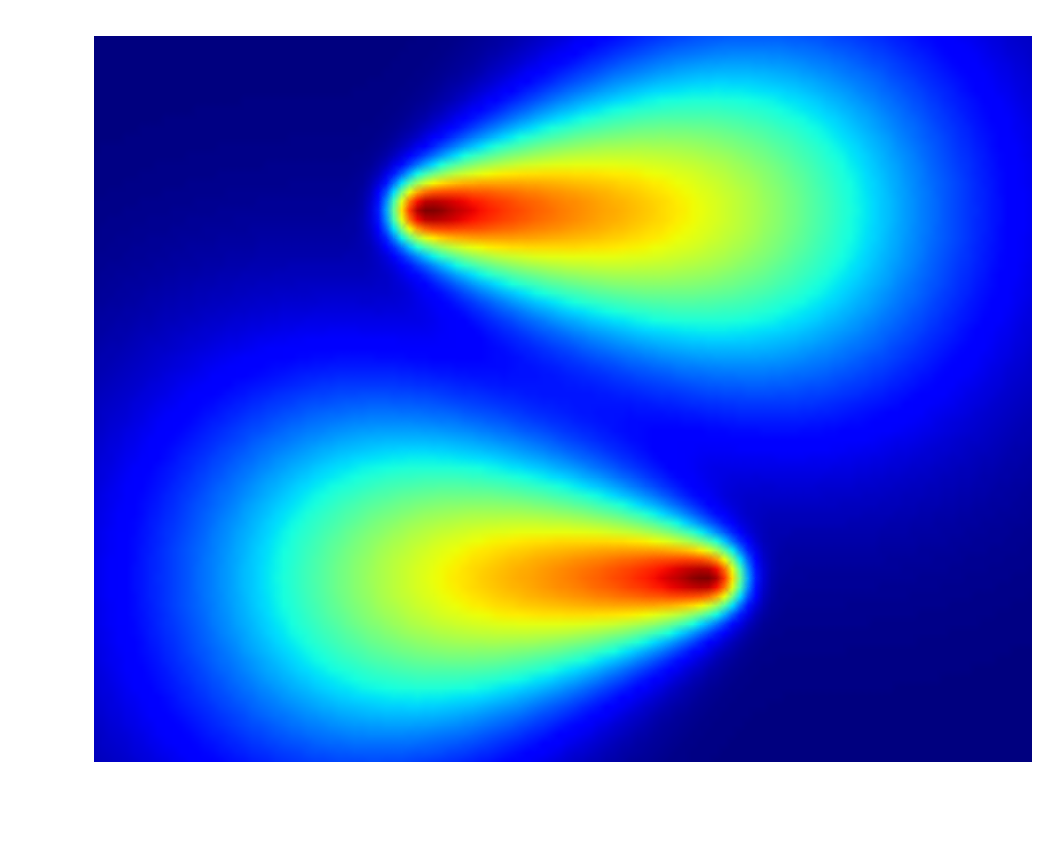
\includegraphics[width=0.24\linewidth]{figs/agent_4} \\
    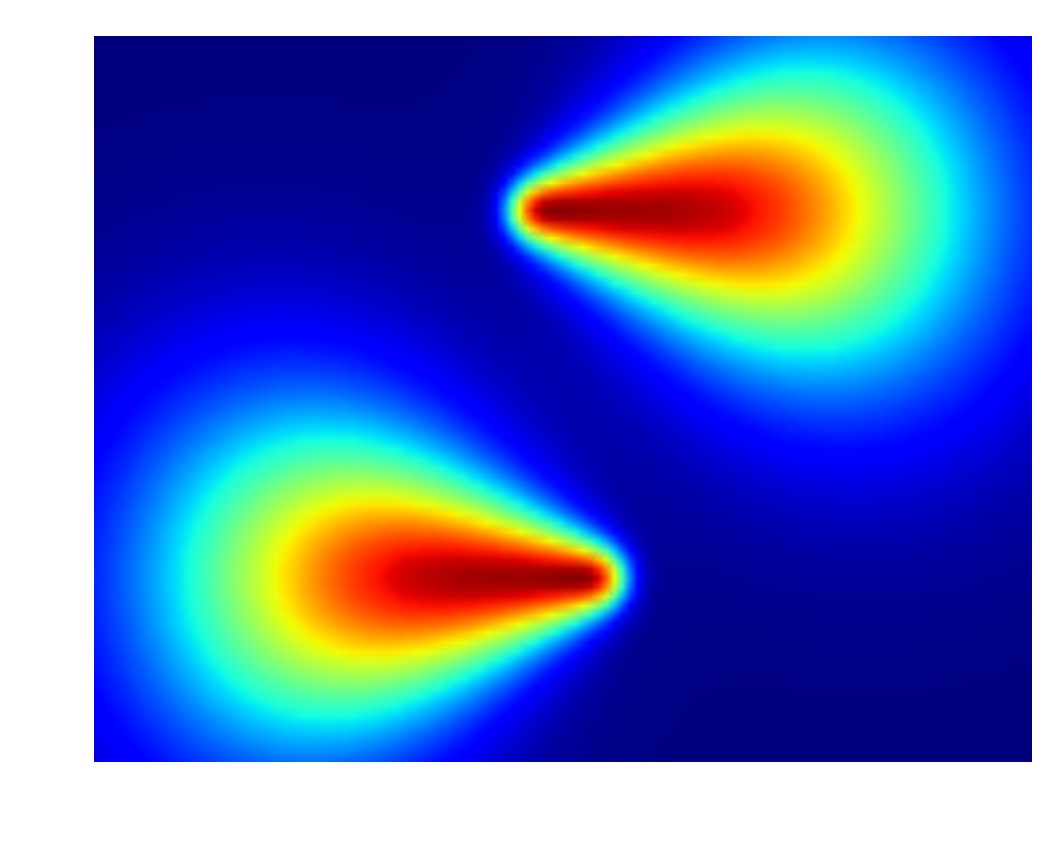
\includegraphics[width=0.24\linewidth]{figs/agent_5}
    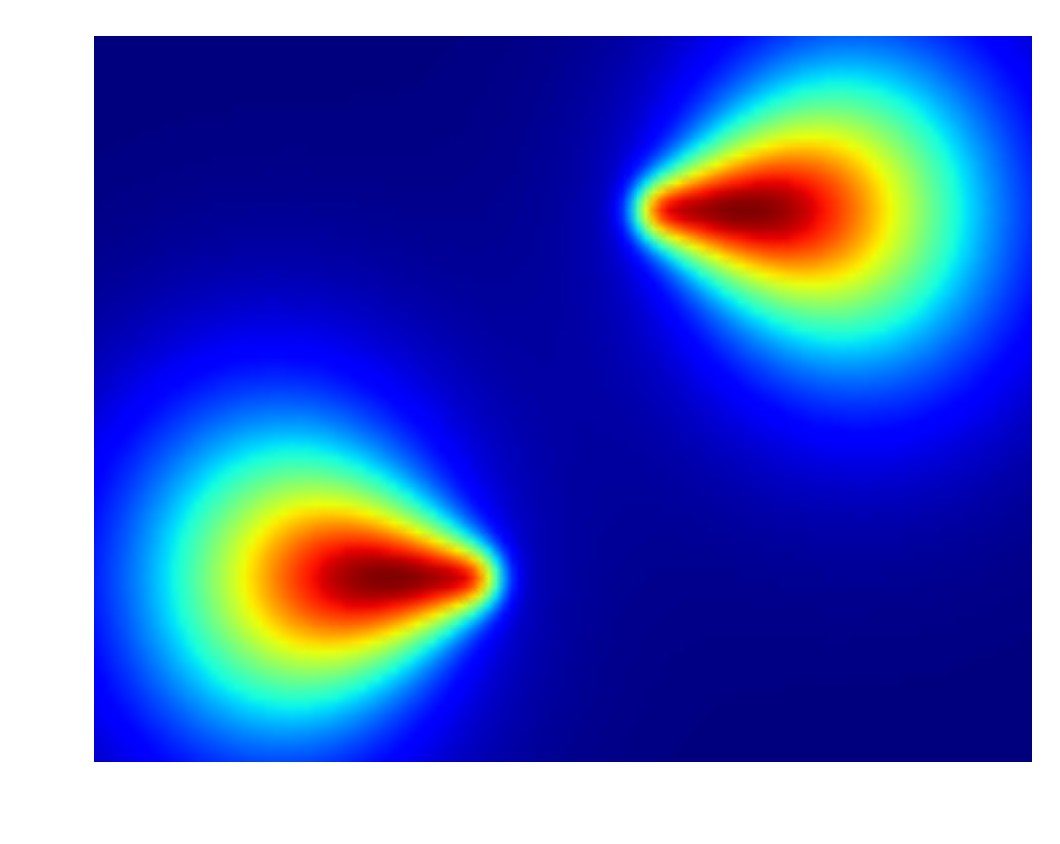
\includegraphics[width=0.24\linewidth]{figs/agent_6}
    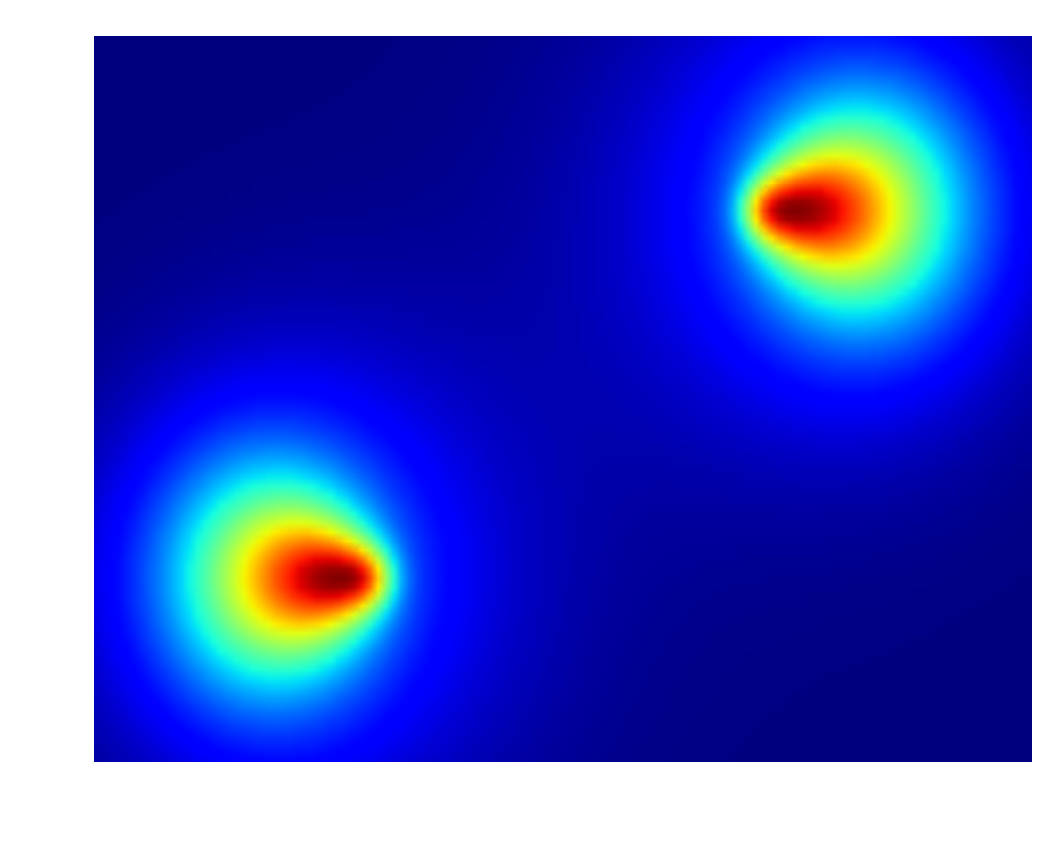
\includegraphics[width=0.24\linewidth]{figs/agent_7}
    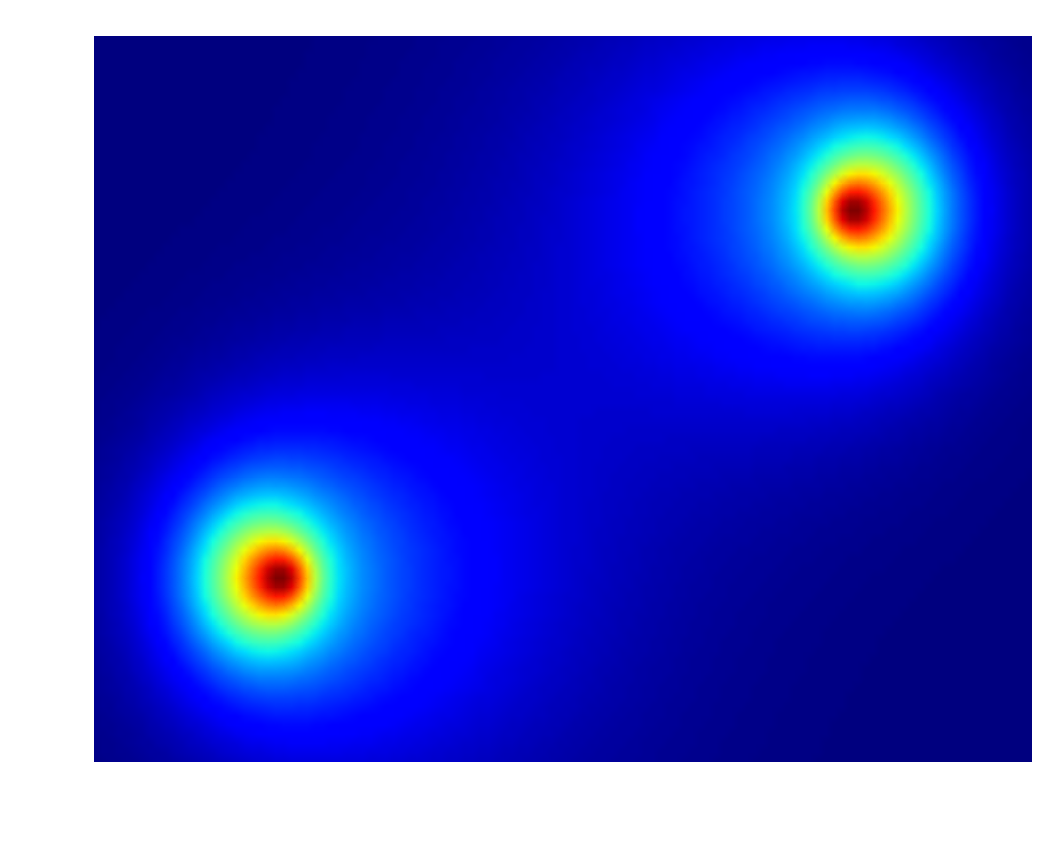
\includegraphics[width=0.24\linewidth]{figs/agent_8}

    \caption{Cost distributions indicating the likelihood that a dynamic
    obstacle will be at a certain location within a given time interval. These
figures show how this distribution changes over time. The sequence progress
from left to right, top to bottom}

    \label{fig:agent_cost}

\end{figure}

\subsubsection{Equations of Motion}

\label{sec:motion}

The motion of a dynamic obstacle is defined by the velocity equation, the
initial configuration, and the amount of uncertainty. Defining the obstacle's
trajectory in terms of its velocity makes it easier to model when creating
scenes. The equation of motion for the dynamic obstacle is shown in
Eq.~\ref{eq:obs_pred}.

\begin{equation}
    \zeta_a(t) =
        \begin{cases}
            \xi_a + \mathlarger{\int_{T_a}^{t}} \dot{\zeta_a}(\lambda) \,
            \mathrm{d}\lambda
            & \text{if } t \geq T_a \\
            \tilde{\zeta_a}(t) & \text{if } t < T_a
        \end{cases}
    \label{eq:obs_pred}
\end{equation}

In Eq.~\ref{eq:obs_pred}, $\tilde{\zeta_a}$ represents the observed trajectory
of the obstacle whereas $\zeta_a$ corresponds to the predicted trajectory of
the obstacle. This disambiguation is needed because the planner needs to be
able to extrapolate the future movements of a dynamic obstacle. The variables,
$\xi_a$ and $T_a$ are initially set to $I_a$ and $0$ respectively and are
dynamically updated when the algorithm replans. The need for this and how it is
designed will be discussed in Sec.~\ref{sec:design_planner}

For the experiments, the motion of the obstacles is simulated by adding a
random variable, $\rho \sim \mathcal{U}(-\epsilon, \epsilon)$ to the trajectory
during the numerical integration of the velocity equation. This form of
stochasticity allows the obstacle to diverge from its specified trajectory
whilst maintaining the same velocity equation. This means that the obstacle
will not exhibit random, Brownian motion around its specified path, but rather
is able to diverge completely. Also, by adding the random variable to the
velocity equation during the numerical integration, the obstacle will not
"jump" to a new location, but will gradually diverge off of its specified path.
The definition of $\tilde{\zeta_a}$ is shown in Eq.~\ref{eq:obs_observed}.  For
this equation, it is assumed that the function only computes a value for any
given time value, $t$, only once.

\begin{equation}
    \tilde{\zeta_a}(t) =
        \begin{cases}
            \tilde{\zeta_a}(t - \delta t) + \dot{\zeta_a}(t) \cdot \delta t
            + \rho
            & \text{if } t > 0 \\
            I_a & \text{if } t = 0
        \end{cases}
    \label{eq:obs_observed}
\end{equation}

In Eq.~\ref{eq:obs_observed}, $\delta t$ is a constant where $\delta t > 0$ and
is used for the numerical integration of the velocity. Numerical integration is
used in order to allow the path to diverge. Since a recursive function is used
for determining the current position of the obstacle, the obstacle's next
location will be determined by its last location, its velocity, and a certain
error factor $\rho$. This will allow the obstacle to exhibit more than simply
Brownian motion along a path and it will be able to diverge completely from its
specified path. This type of uncertainty is important because it is exhibited
in real-world scenarios such as error propagation in controls and by simply not
having enough information about the actual velocity equation for a given
obstacle. The full extent of $\tilde{\zeta_a}$ is not known by the planner and
this equation is only used to simulate the motion of the obstacles for
experimentation and evaluation of the developed planner.

By increasing the level of stochasticity, $\epsilon$, for a given dynamic
obstacle, it will be more likely to diverge from its current path. This means
that the uncertainty of a given dynamic obstacle can be parametrized by its
value for $\epsilon$.

The motion of a dynamic obstacle is described by it's velocity and a starting
location in order for the planner to be able to continue to predict an
obstacle's motion even when it diverges from its current path. If the
obstacle's motion was described by parametric equations of its position, it
would not be possible to continue to predict where it is going to move once it
is no longer following its prescribed path since the obstacle may diverge from
this path completely.

\subsubsection{Available Information}

It is important to note what information is available to the planner. It is not
assumed that the planner has perfect information about the motion of the
obstacles or their associated definitions. The planner only has access to the
obstacles' velocity equations and their positions throughout the execution of
path.  The planner does not know the amount of noise, $\epsilon$, being
injected into the obstacles' velocities as described in Sec.~\ref{sec:motion}.
It is also assumed that the robot or an external system is evaluating the cost
distribution based on the predicted motion of the dynamic obstacles in the
future. Even though these assumptions may seem unrealistic, there are currently
methods being developed that are able to extrapolate and predict the motion of
obstacles based on their past locations or based on the algorithm used to
dictate their behaviour~\cite{rus, cmu, boulder, edi1, edi2, keeper}. Also, as
described in Sec.~\ref{sec:plannerdiscussion}, the planner does not need to
have a perfectly precise equation for the obstacles' motion because the planner
has the ability to construct a new plan through the environment if the
prediction of the obstacles' motion does not accurately depict where the actual
location of the obstacle.

\subsection{Planning Algorithm}

\label{sec:design_planner}

The planning algorithm for Dodger has three major components. First, a two
dimensional probabilistic roadmap is constructed over the search space in order
to capture the spatial connectivity of the environment. The planner then uses a
best-first (BestFS) graph search algorithm to determine the safest path from
the initial position to the goal position by creating a temporal search tree
through the graph in order to account for time-dependent edge costs. Once the
robot has an initial path to follow, it will incrementally pursue this path
whilst updating its information about the location of the dynamic obstacles. If
any of the obstacles deviate from their predicted path, the planner will
generate a new path (replan) for the robot using this information. These three
components allow the planner to reduce the number of samples over time by
reusing the same two dimensional roadmap and allows the planner to account for
dynamic obstacles with stochastic motion by replanning. These are improvements
to the first sampling based technique described in Sec.~\ref{sec:stroadmap}

\subsubsection{Building the Roadmap}

The first component of the planning algorithm is the underlying two dimensional
roadmap which represents the spatial connectivity of the environment. This
roadmap is constructed using a standard variant of the probabilistic roadmap
algorithm created by Kavraki et al~\cite{prm}. A probabilistic roadmap is a
undirected graph, $(V, E)$, created by randomly sampling $n$ configurations in
the configuration space of the robot and connecting them such that if $(i, j)
\in E$, then $||i - j|| < d$, both $i$ and $j$ are not within any of the static
obstacles, and there is no collision along the geometric edge from $i$ to $j$.
In this work the configuration space is $\mathbb{R}^2$ and the edge between two
nodes is a straight line. The nodes in the roadmap represent the possible
configurations of the robot and in this work, points along the edge between two
nodes represent geometric transitions from one node to another. The complexity
of the graph is parametrized by the number of samples, $n$, and the maximum
distance between nodes, $d$. By increasing the number of samples, the density
of samples increases and therefore the average degree for a node in the graph
increases.  Likewise, if the maximum distance between nodes increases, so does
the average degree for a node in the graph.  Pseudocode is provided for
constructing a probabilistic roadmap in Algo.~\ref{algo:prm}.

% Algorithm to generate a roadmap
\begin{algorithm}[ht]
    \caption{$\Function{Roadmap}(n, d, w, h, O)$}
    \algorithmicrequire{
        \\$n$: Maximum number of samples
        \\$d$: Maximum distance between neighbouring nodes
        \\$w$: Height of the scene
        \\$w$: Width of the scene
        \\$O$: Set of obstacles
    }
    \\\algorithmicensure{
        \\An unweighted graph of points describing the
        connectivity of the environment
    }
    \label{algo:prm}
    \begin{algorithmic}[1]
        \setcounter{ALC@line}{0}
        \vspace*{1mm}

        \FOR{$k = 1$ \TO $n$}
            \STATE $q \leftarrow \Function{RandomPoint2D}(w, h)$
            \IF{$\bigwedge_{o \in O} \neg \Function{Collision}(o, q)$}
                \STATE $V \leftarrow V \cup \{q\}$
            \ENDIF
        \ENDFOR

        \FORALL{$i \in V$}
            \FORALL{$j \in V$}
            \IF{$i \neq j \wedge ||i - j|| \leq d \wedge
                \bigwedge_{o \in O} \neg \Function{Collision}(o, i, j)$}
                    \STATE $E \leftarrow E \cup \{(i, j)\}$
                \ENDIF
            \ENDFOR
        \ENDFOR
        \RETURN $(V,E)$
    \end{algorithmic}
\end{algorithm}

% text below is most likely redundant, like this comment

In Algo.~\ref{algo:prm}, first at most $n$ points are sampled and added to the
set of vertices, $V$, if and only if there is not a collision with any of the
static obstacles. Essentially the Cartesian square of $V$ is iterated over and
any two points that are not the same, whose distance is less than $d$, and if
there is no collision along the edge between these two points are added to the
edge set, $E$. Finally, the vertices and edges are returned as a tuple
representing the graph. Fig.~\ref{fig:prm} shows a constructed probabilistic
roadmap with 300 nodes.

\begin{figure}[h!]
    \centering
    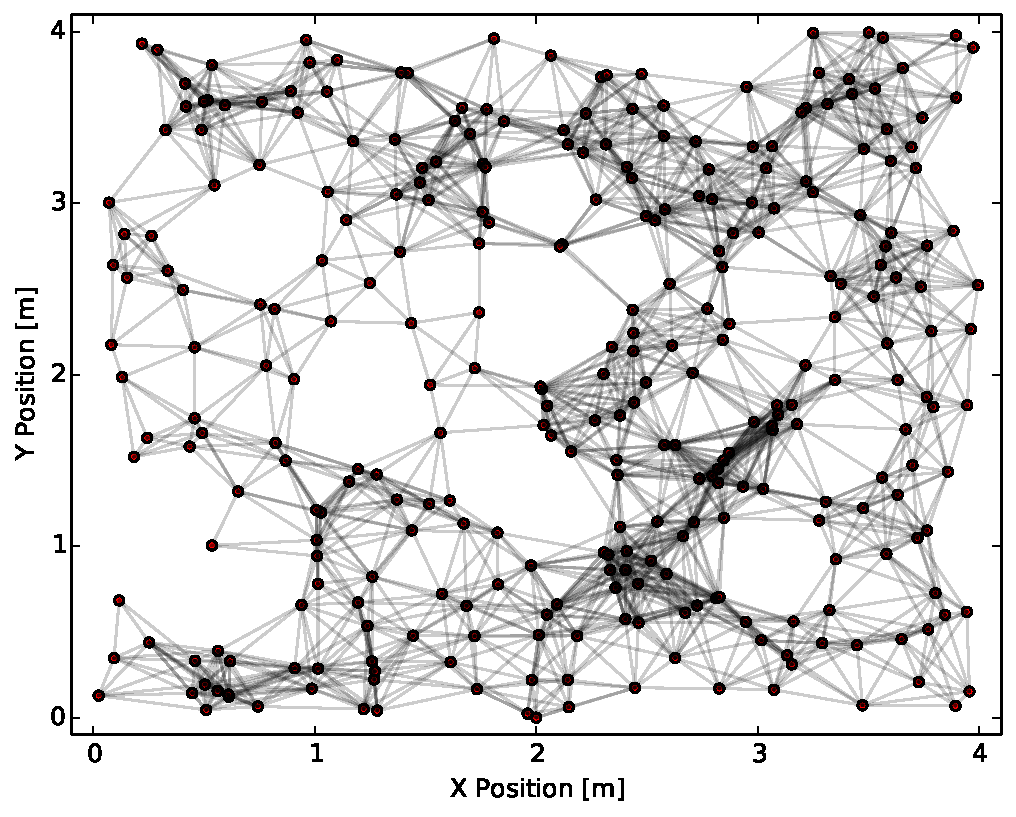
\includegraphics[width=0.8\linewidth]{figs/roadmap}

    \caption{An example of a probabilistic roadmap generated in free space
    without the presence of obstacles. The nodes are represented by the circles
and the red line as the edges between the nodes.}

    \label{fig:prm}
\end{figure}

\subsubsection{Searching the Graph}

To search the generated two dimensional probabilistic roadmap in space-time, a
novel best first search ($\Acronym{tBestFS}$) algorithm has been developed that
creates a search tree that expands the current node not only in space but also
in time until the current node is within an acceptance radius the goal. This
algorithm works by using a priority queue to store the expanded nodes. The
priority is based on two things, how many times a two dimensional node in the
probabilistic roadmap has been expanded and the cost to reach the node in
space-time in the queue. A dictionary indexed by the node and mapped to an
integer is used to keep track of how many times the node has been visited. The
cost between two nodes in space-time, $(i, t)$ and $(j, t')$ is defined by the
line integral from $i$ to $j$ over the exponential of the cost distribution $P$
for the time interval $[t_0, t_m]$ and set of dynamic obstacles $A$. This
function uses the exponential of the cost distribution in order to emphasize
higher costs along the path. This is formally shown in Eq.~\ref{eq:cost}.

% Graph cost function

\begin{align}
    C(i, j, t_0, t_m, A) &= \int^1_0 \exp{\Big(
        P(x(\lambda), y(\lambda), t_0, t_m, A) + 1 \Big)
    } \cdot \sqrt{\Big(\frac{\dif x}{\dif t}\Big)^2
    + \Big(\frac{\dif y}{\dif t}\Big)^2}
    \,\mathrm{d}\lambda \notag \\
    % ----------------------------------------------
    &= \int^1_0 \exp{\Big(
        P(x(\lambda), y(\lambda), t_0, t_m, A) + 1 \Big)
    } \cdot \sqrt{(j_x - i_x)^2 + (j_y - i_y)^2}
    \,\mathrm{d}\lambda \notag \\
    % ----------------------------------------------
    &= \int^1_0 \exp{\Big(
        P(x(\lambda), y(\lambda), t_0, t_m, A) + 1 \Big)
    } \cdot ||i - j|| \,\mathrm{d}\lambda
    \label{eq:cost}
\end{align}

In Eq.~\ref{eq:cost}, $C$ is a function $C: \R^2 \times \R^2 \times (\R^+)^2
\times (\R^+)^2 \times \mathcal{A} \rightarrow \R$ where $\mathcal{A}$ is the
set of all possible sets of dynamic obstacles, and $x(\lambda) = (j_x - i_x)
\cdot \lambda + i_x$ and $y(\lambda) = (j_y - i_y) \cdot \lambda + i_y$ are the
parametric equations of the line from $i$ to $j$.  Eq.~\ref{eq:cost} increases
exponentially as the maximum cost along the line increases and therefore makes
edges with larger maximum costs more costly than edges with lower maximum
costs. To combine the two cost formulations for an edge, $((i, t), (j, t'))$, a
weighted sum is computed that adds the number of times node $j$ has been
visited with the line integral over the cost distribution from $i$ to $j$ for
the given time interval. This total cost function is formally described in
Eq.~\ref{eq:totalcost}.

\begin{equation}
    TC(i, j, t_0, t_m, A, D) = \psi \cdot C(i, j, t_0, t_m, A) +
    \omega \cdot D_j
    \label{eq:totalcost}
\end{equation}

In Eq.~\ref{eq:totalcost}, $\psi$ and $\omega$ are scaling constants. It is
important to incorporate a penalty for returning to a location that has already
been visited even if this penalty is small because the tBestFS algorithm may
choose to only expand nodes in a safe area and thus not reach the goal since
there is not a heuristic to sample nodes closer to the goal in order give
preference to safer paths instead of shorter ones.

Since the algorithm operates in both space and time, the search tree is
expanded at a given node, $i$ at a time $t$, by determining how long it would
take the robot to reach all of the neighbours of $i$ and not only adding each
neighbour of $i$ into the priority queue with its associated cost, but also
adding the time at which the robot would reach each neighbour. This is
accomplished by assuming the robot will travel at a constant speed, $s$,
through the environment which makes it easy to compute how long it would take
the robot to reach a neighbour, $j \in \Function{Neighbours}(i)$. The time it
would take for the robot to reach a neighbour, $j$ from $i$ is $||i - j|| / s$
which would make the robot reach $j$ at time $t + ||i - j|| / s$.  Also, since
the algorithm is also operating in time, the robot is able to stay at the same
location for a given wait time $\delta t$ if it is less costly than moving
forward to any of its neighbours.

The algorithm progresses forward by expanding the best current node in the
priority queue. This is the node that has the smallest combined cost in the
queue.  Once a node, $i$ at time $t$, is expanded and its temporal neighbours
determined, the parent for each of these neighbours is defined as $i$ at time
$t$. By storing the parents of each of the neighbours, it becomes possible to
backtrack from the goal to the starting position once the goal is reached and
construct a path to the goal configuration. The algorithm terminates either
when there are no more nodes in the priority queue or once the node popped out
of the queue is less than a certain distance away from the goal node. Once the
node popped out of the priority queue is within the goal region, the path to
the goal is returned. The algorithm used for searching the graph is described
formally in Algo.~\ref{algo:search}.

% Algorithm to search the graph
\begin{algorithm}[ht]
    \caption{$\Acronym{tBestFS}(V, E, R, A, p, g, T)$}
    \algorithmicrequire{
        \\$V$: Set of vertices
        \\$E$: Set of edges
        \\$R$: Goal radius
        \\$A$: Set of dynamic obstacles
        \\$p$: Starting point of the robot
        \\$g$: Goal point for the robot
        \\$T$: Time at which the search should start
    }
    \\\algorithmicensure{
        \\A temporal path from the initial configuration of the robot
        to the goal configuration
    }

    \label{algo:search}
    \begin{algorithmic}[1]
        \setcounter{ALC@line}{0}
        \vspace*{1mm}
        \STATE $Q \leftarrow \Function{PriorityQueue}()$
        \STATE $D \leftarrow \Function{Dictionary}()$
        \STATE $\mathcal{P} \leftarrow \Function{Dictionary}()$
        \STATE $\Function{Insert}(Q, p, T)$
        \WHILE {$|Q| > 0$}
            \STATE $(q, t) \leftarrow \Function{Pop}(Q)$
            \IF{$||q - g|| \leq R$}
                \RETURN $\Function{BacktrackPath}(p, q, t, \mathcal{P})$
            \ENDIF
            \STATE $S \leftarrow \emptyset$
            \STATE $N \leftarrow \Function{Neighbours}(V, E, q) \cup \{q\}$
            \FORALL {$n \in N$}
                \IF {$q \neq n$}
                    \STATE $t' \leftarrow ||q - n|| / s + t$
                \ELSE
                    \STATE $t' \leftarrow t + \delta t$
                \ENDIF
                \STATE $\mathcal{P}_{(n, t')} \leftarrow (q, t)$
                \STATE $c \leftarrow \psi \cdot C(q, n, t, t', A) + \omega
                    \cdot D_{n}$
                \STATE $D_{n} \leftarrow D_{n} + 1$
                \STATE $Q \leftarrow \Function{Insert}(Q, (n, t'), c)$
            \ENDFOR
        \ENDWHILE
    \end{algorithmic}
\end{algorithm}

From the algorithm in Algo.~\ref{algo:search}, it is evident that picking a
good wait time, $\delta t$, is important for generating safe paths through the
environment. Having a large value for $\delta t$ can lead to very suboptimal
paths because even though staying in the same position for a given period of
time may be safer than moving to any of the neighbours, staying there for too
long could lead the planner to miss safer viable paths. For instance, say the
planner has expanded a node, $i$ at time $t$ and $TC(i, i, t, t + \delta t, A,
D) < TC(i, j, t, t + ||i - j|| / s, A, D)$ for all $j \in
\Function{Neighbours}(i)$. There may be a neighbour $j$ and some time $t'$ such
that $t < t' < t + \delta t$ where $TC(i, j, t, t', A, D) < TC(i, i, t, t +
\delta t, A, D)$. Moving the robot to node $j$ at time $t'$ from $i$ at time
$t$ would lead to a safer path than staying at node $i$ until time $t + \delta
t$. This is why it is important for the safety of the generated paths to use a
small value for $\delta t$ in order to not miss sampling safe paths. By using a
smaller value for $\delta t$, the chance that a safer path would be missed
decreases, but the number of nodes in the search tree would increase.

Fig.~\ref{fig:tree} shows how the search tree for $\Acronym{tBestFS}$ is being
built in space-time as the algorithm progresses. The sequence for this figure
is left to right, up to down. The last plot in the Fig.~\ref{fig:tree} also
shows the path in red that was returned by $\Acronym{tBestFS}$.
Fig.~\ref{fig:ex_agents} shows how the dynamic obstacle cost distribution
changes over time for the search tree in Fig.~\ref{fig:tree}. In
Fig.~\ref{fig:tree}, the tree is being expanded into areas that have low cost
in space-time and that is why the tree is being expanded on the left of the
scene. It is evident that the tree is essentially moving around the dynamic
obstacles when they are all near each other on the right side of the scene.

\begin{figure}[h!]
    \centering
    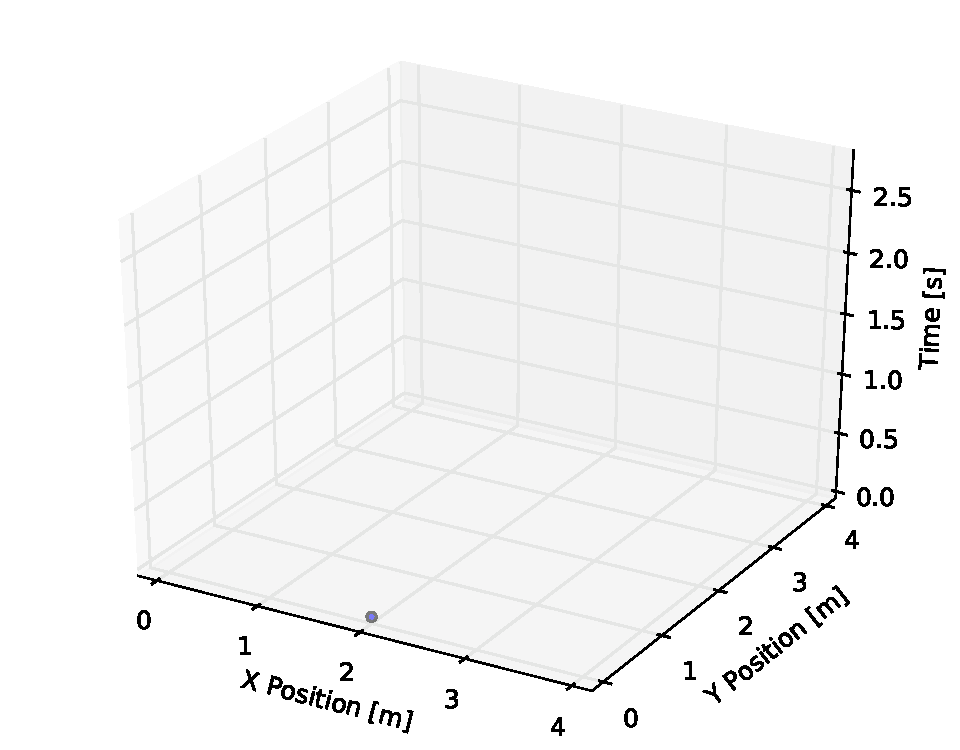
\includegraphics[width=0.32\linewidth]{figs/tree_0}
    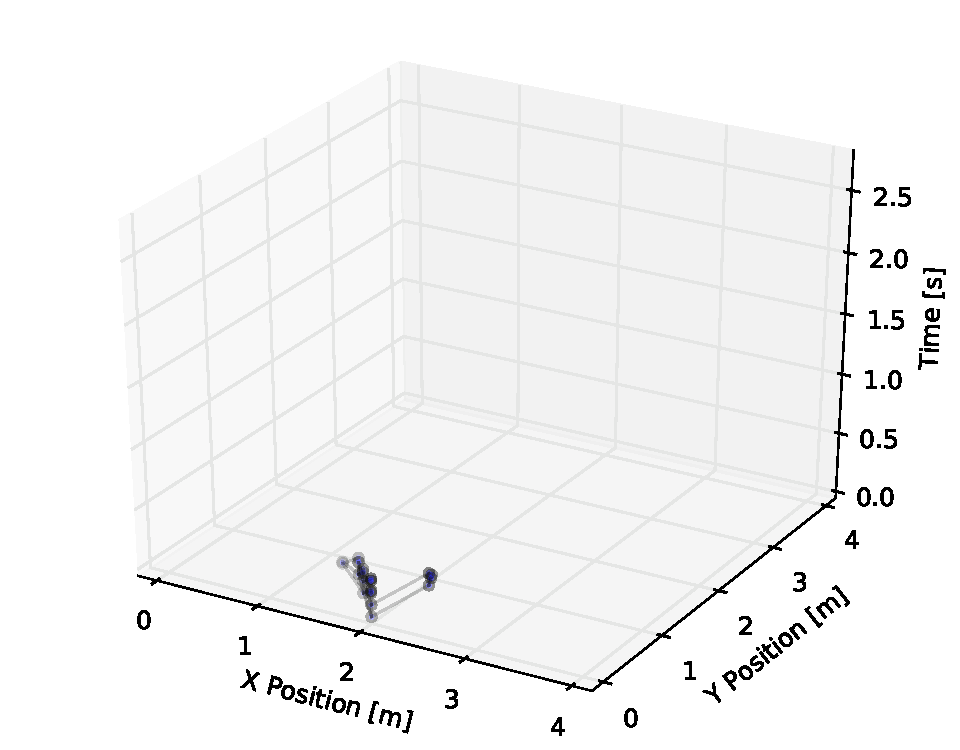
\includegraphics[width=0.32\linewidth]{figs/tree_1}
    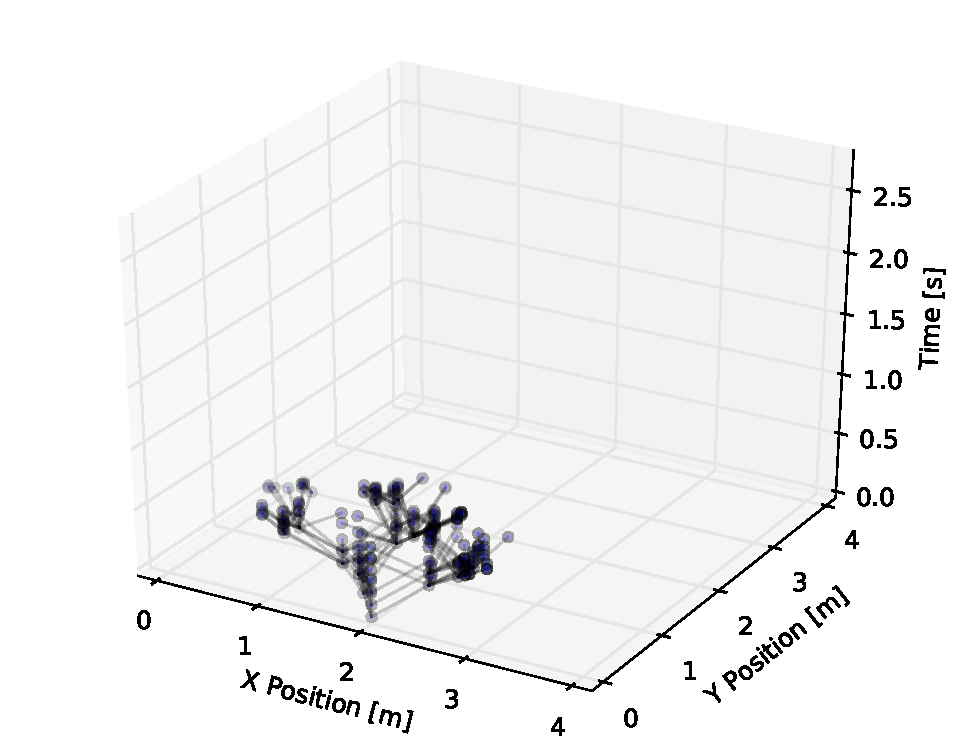
\includegraphics[width=0.32\linewidth]{figs/tree_2} \\
    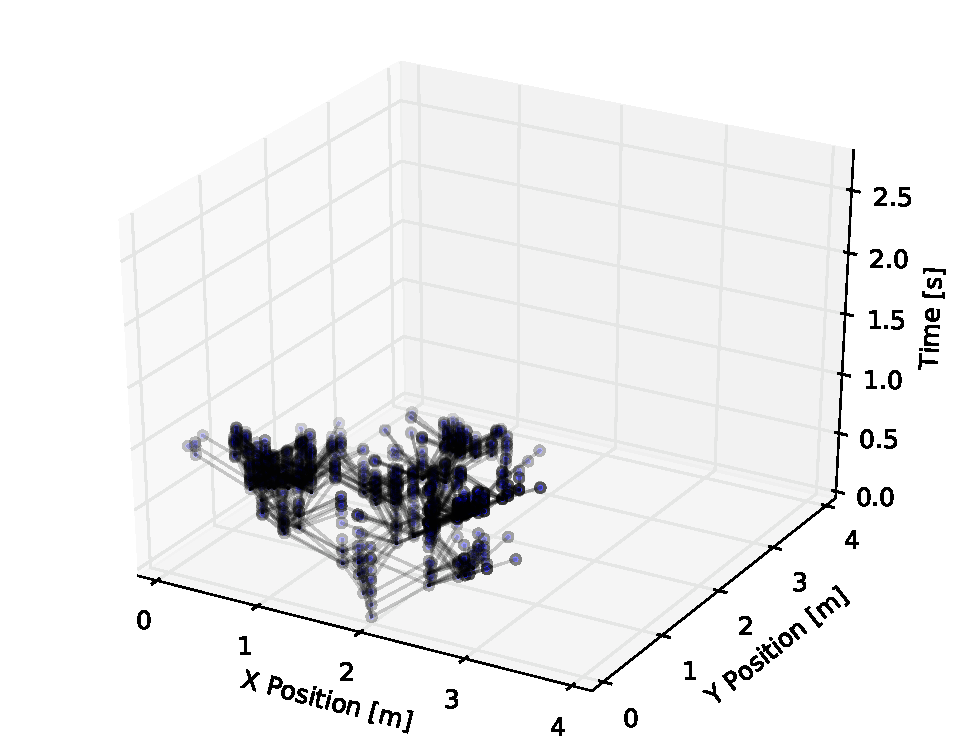
\includegraphics[width=0.32\linewidth]{figs/tree_3}
    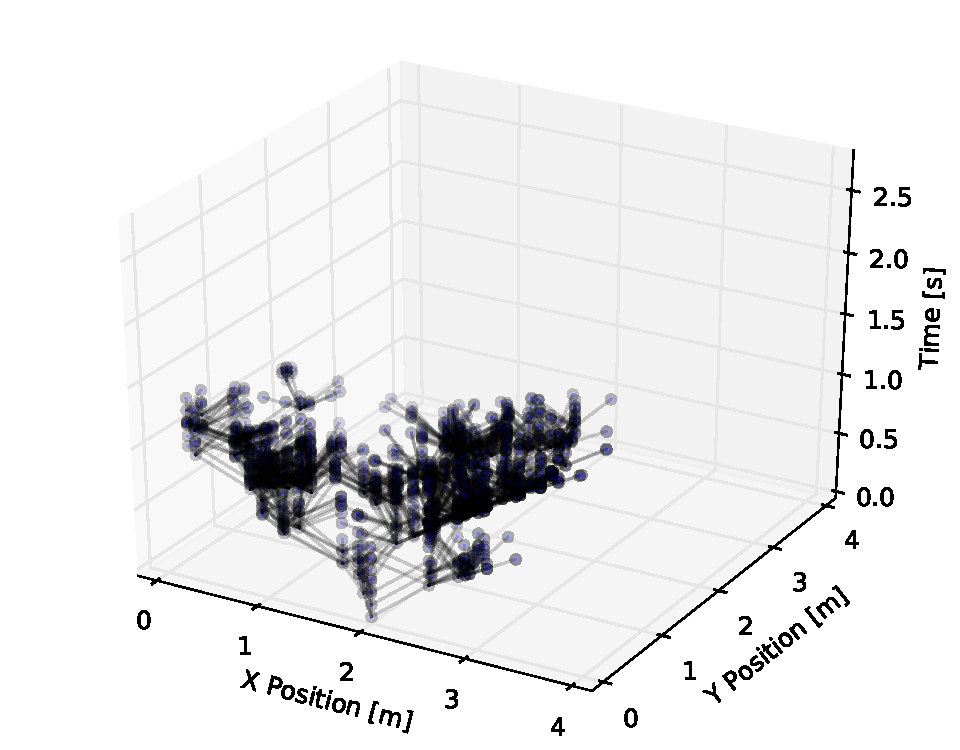
\includegraphics[width=0.32\linewidth]{figs/tree_4}
    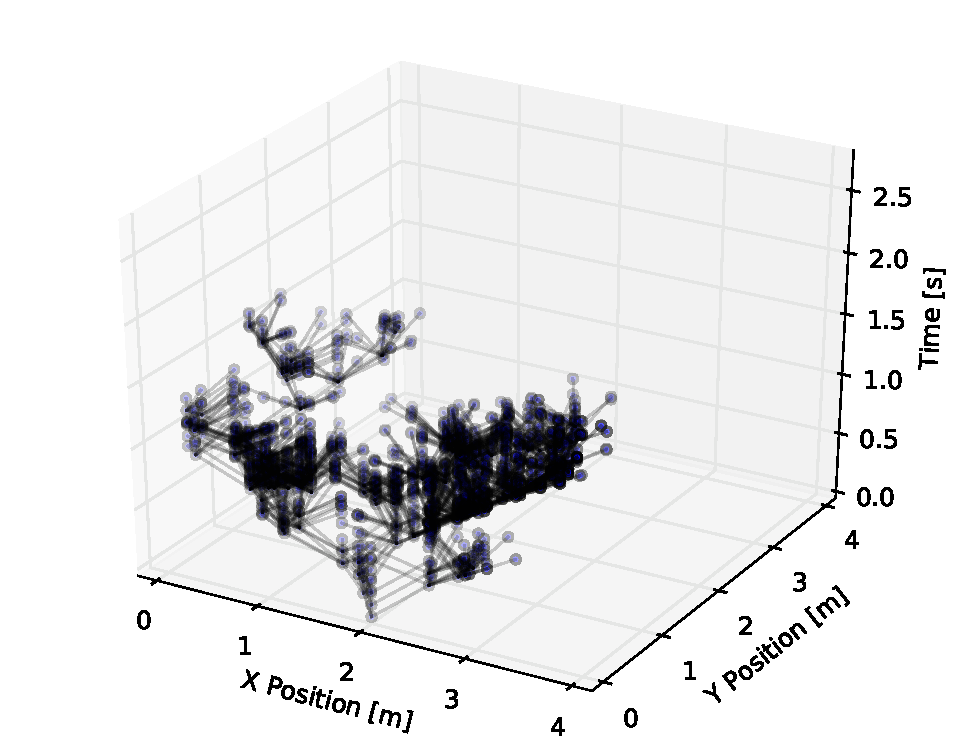
\includegraphics[width=0.32\linewidth]{figs/tree_5} \\
    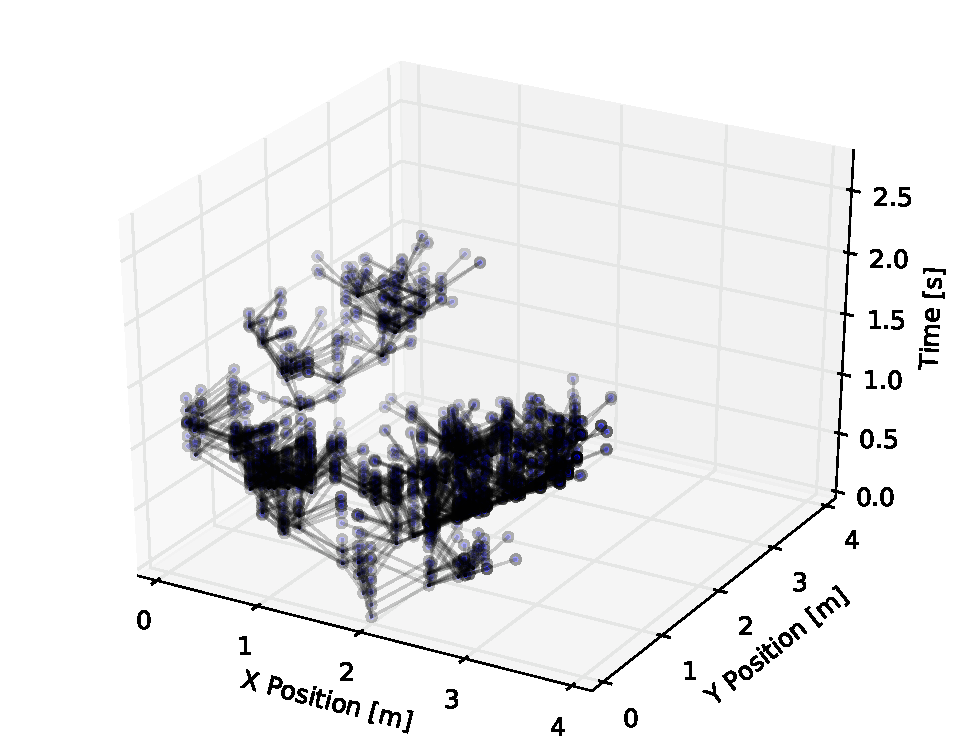
\includegraphics[width=0.32\linewidth]{figs/tree_6}
    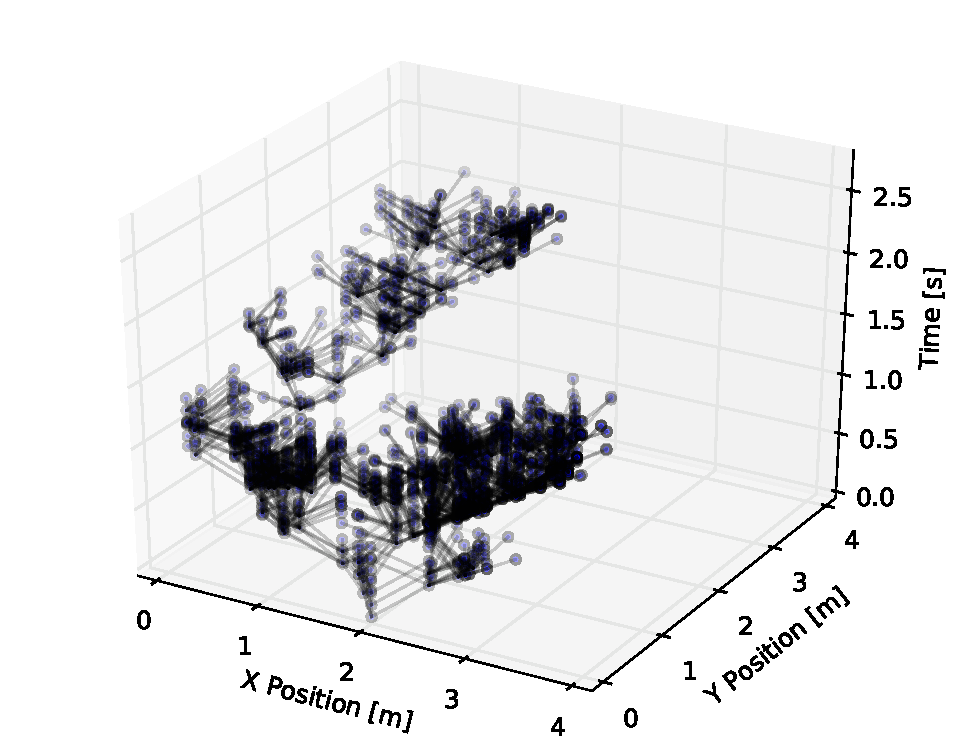
\includegraphics[width=0.32\linewidth]{figs/tree_7}
    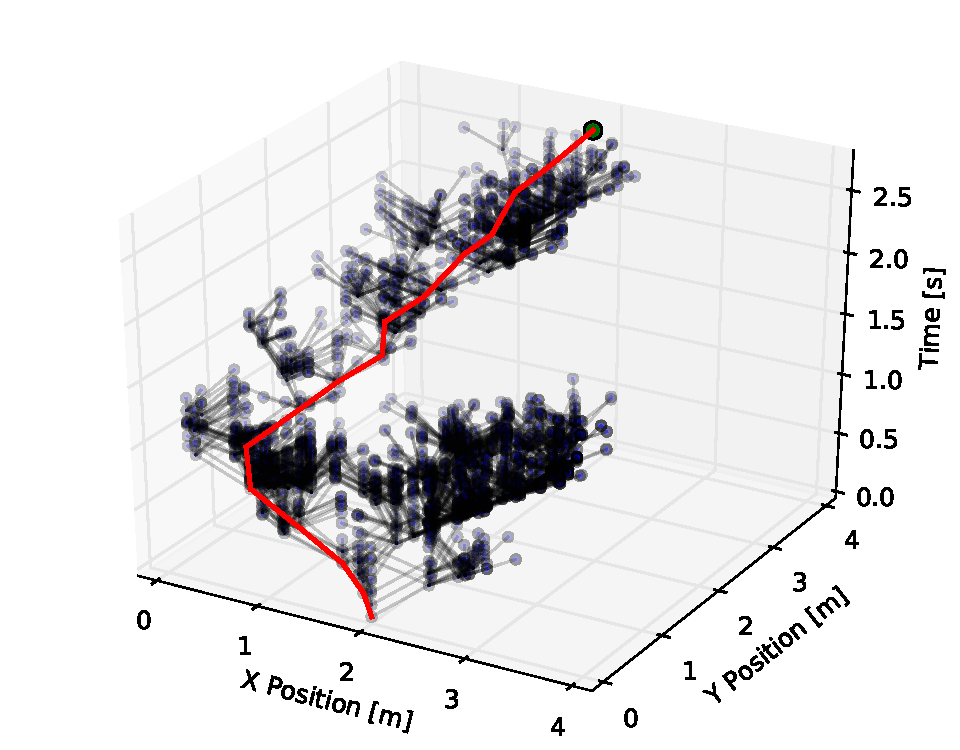
\includegraphics[width=0.32\linewidth]{figs/tree_8}

    \caption{A depiction of the search tree generation for a given
    probabilistic roadmap. The $x$ and $y$ axes represent the $x$ and $y$
location of the node, and the vertical axis represents time. The sequence
progress from left to right, up to down. The final image in sequence also shows
the path taken by the robot in red.}

    \label{fig:tree}
\end{figure}

\begin{figure}[h!]
    \centering
    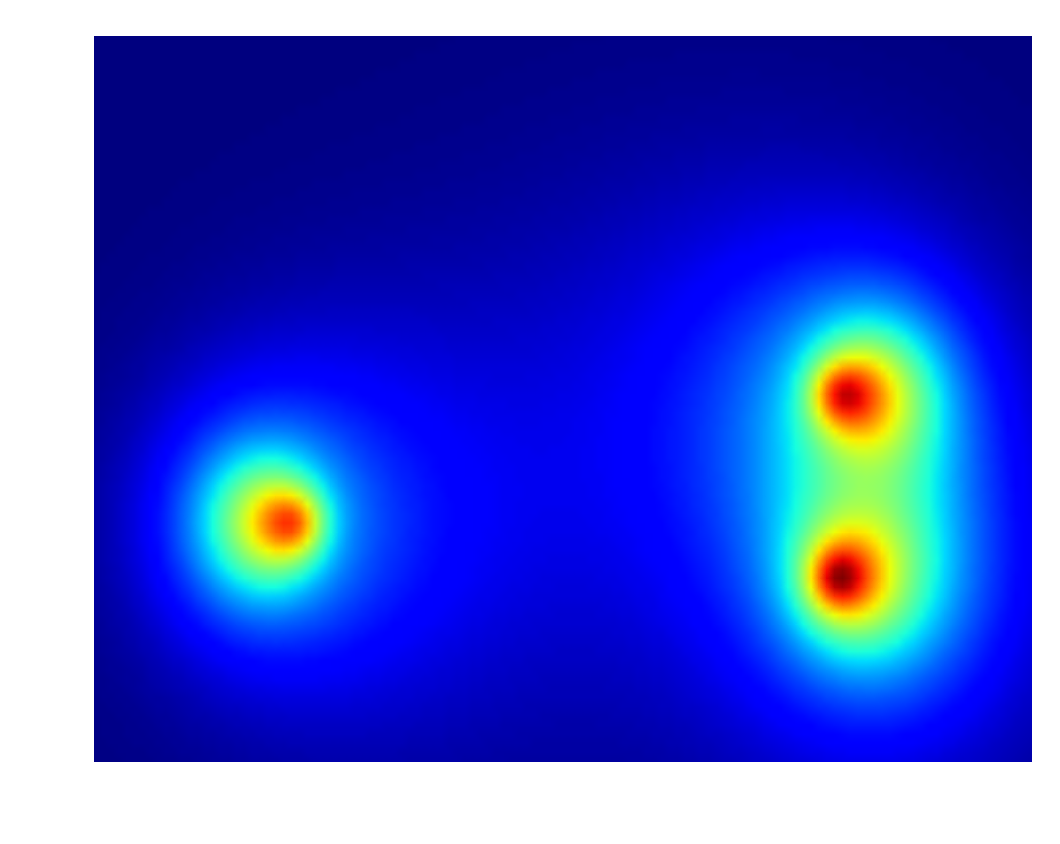
\includegraphics[width=0.32\linewidth]{figs/ex_agent_0}
    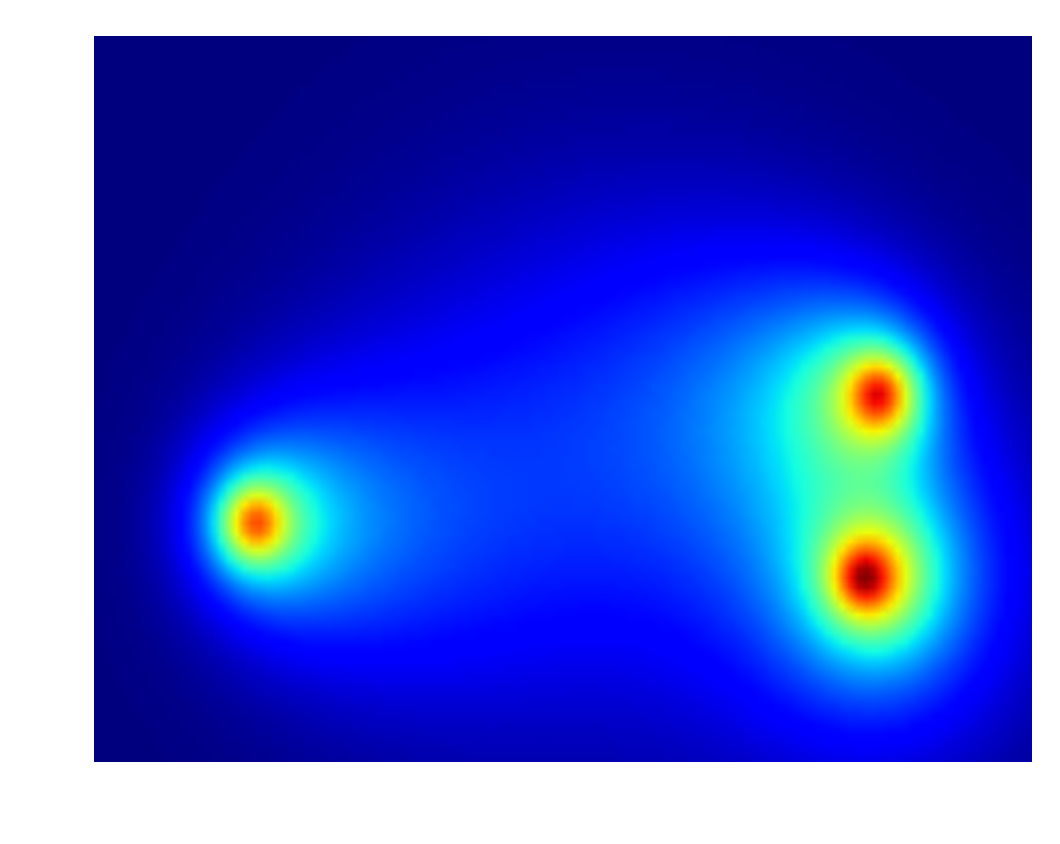
\includegraphics[width=0.32\linewidth]{figs/ex_agent_1}
    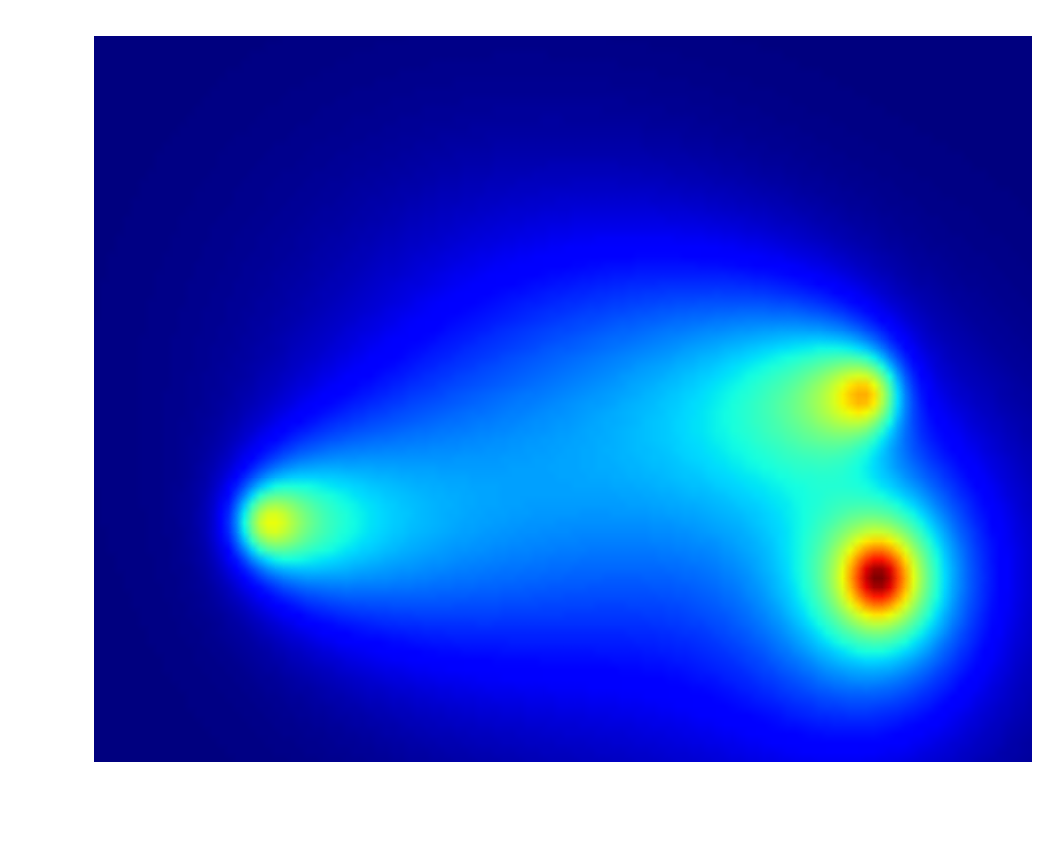
\includegraphics[width=0.32\linewidth]{figs/ex_agent_2} \\
    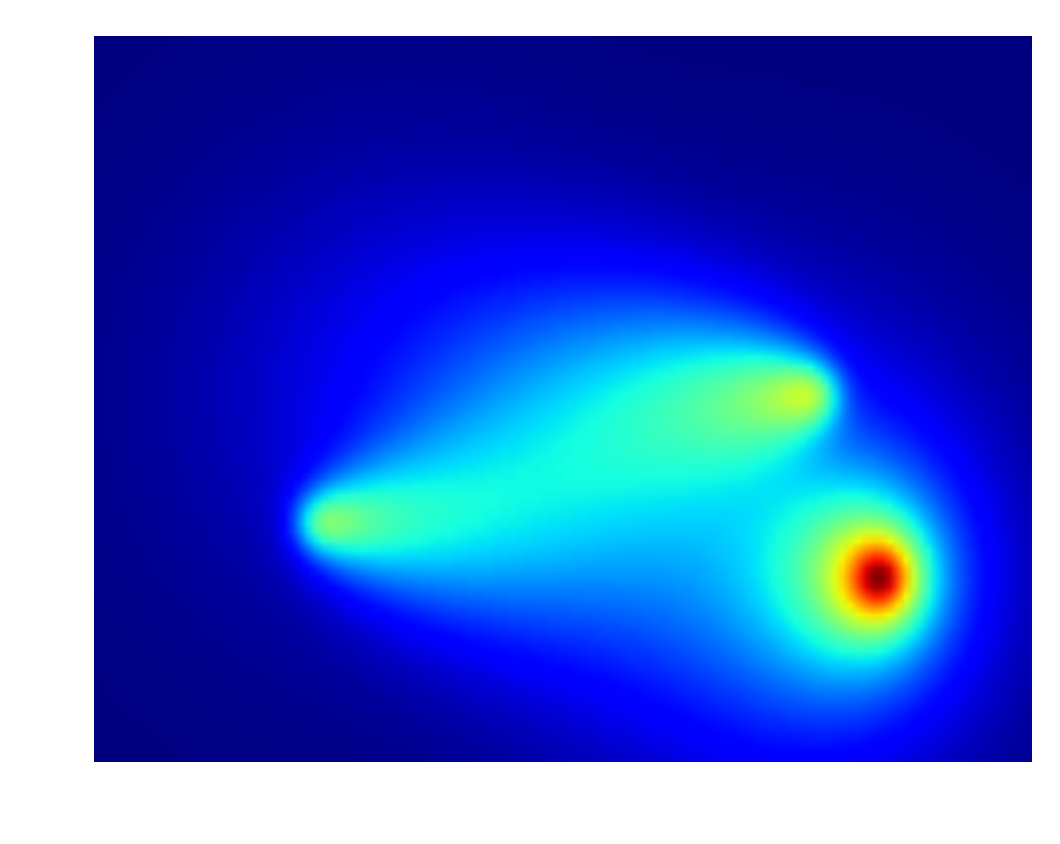
\includegraphics[width=0.32\linewidth]{figs/ex_agent_3}
    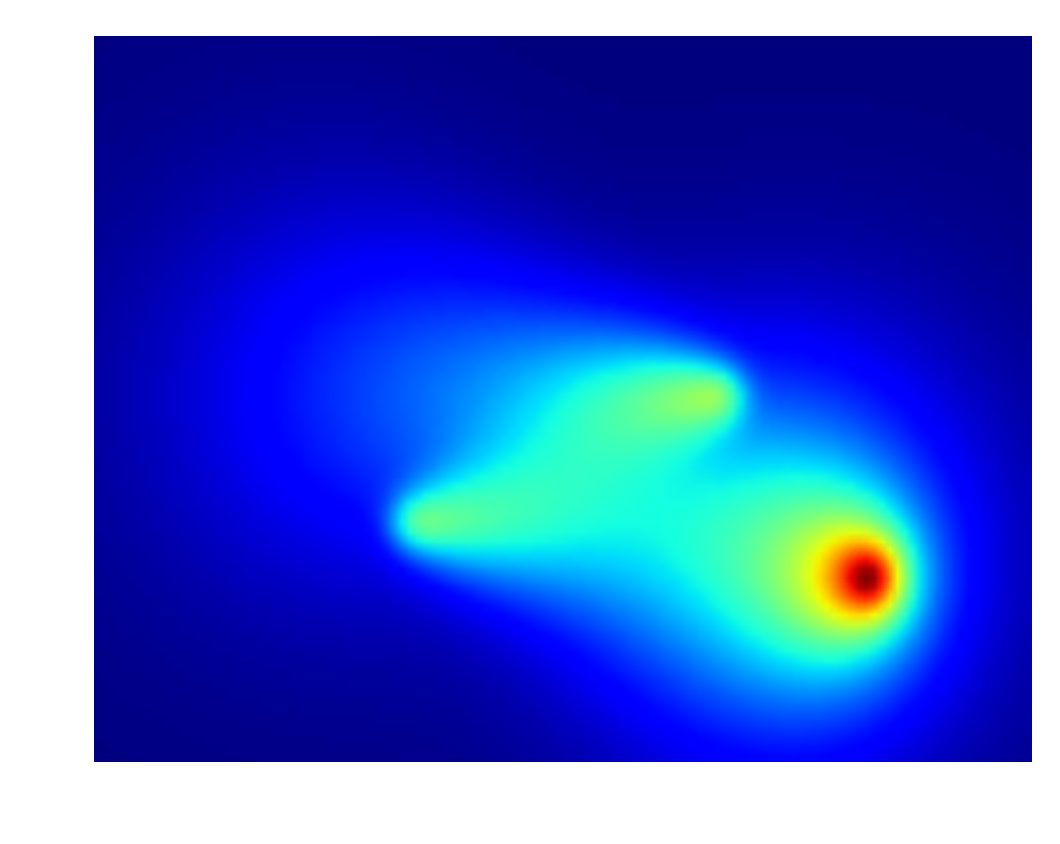
\includegraphics[width=0.32\linewidth]{figs/ex_agent_4}
    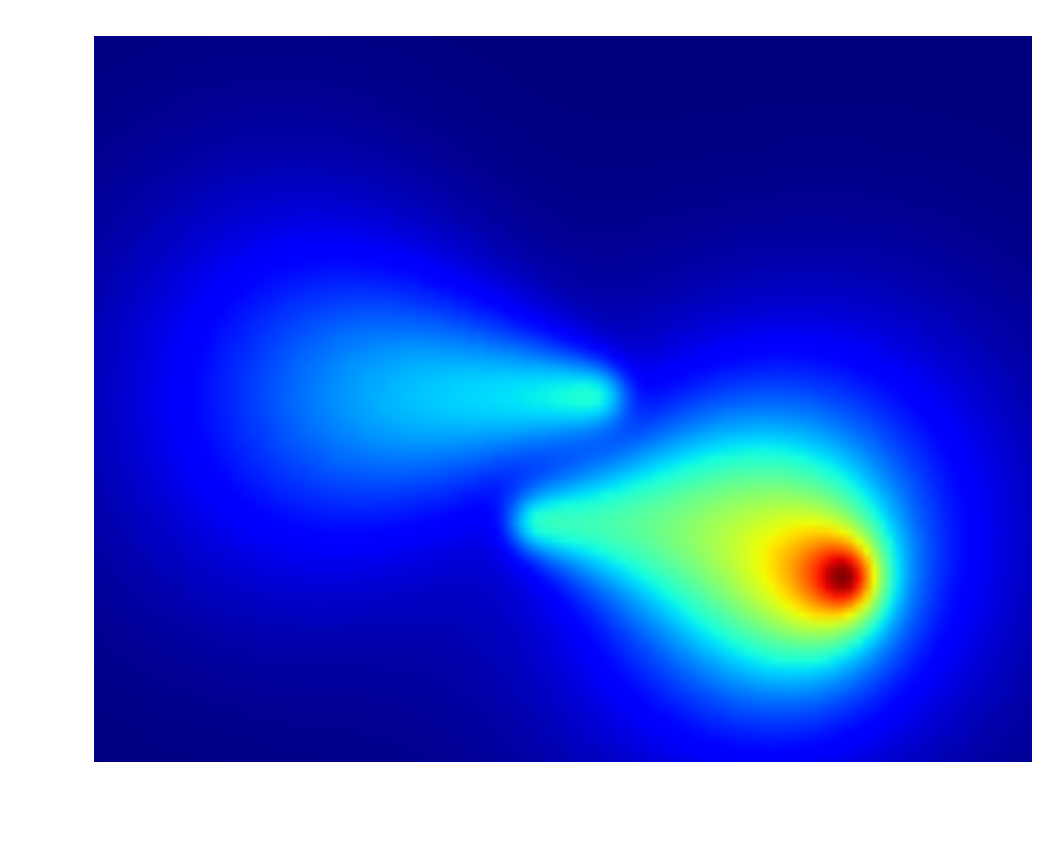
\includegraphics[width=0.32\linewidth]{figs/ex_agent_5} \\
    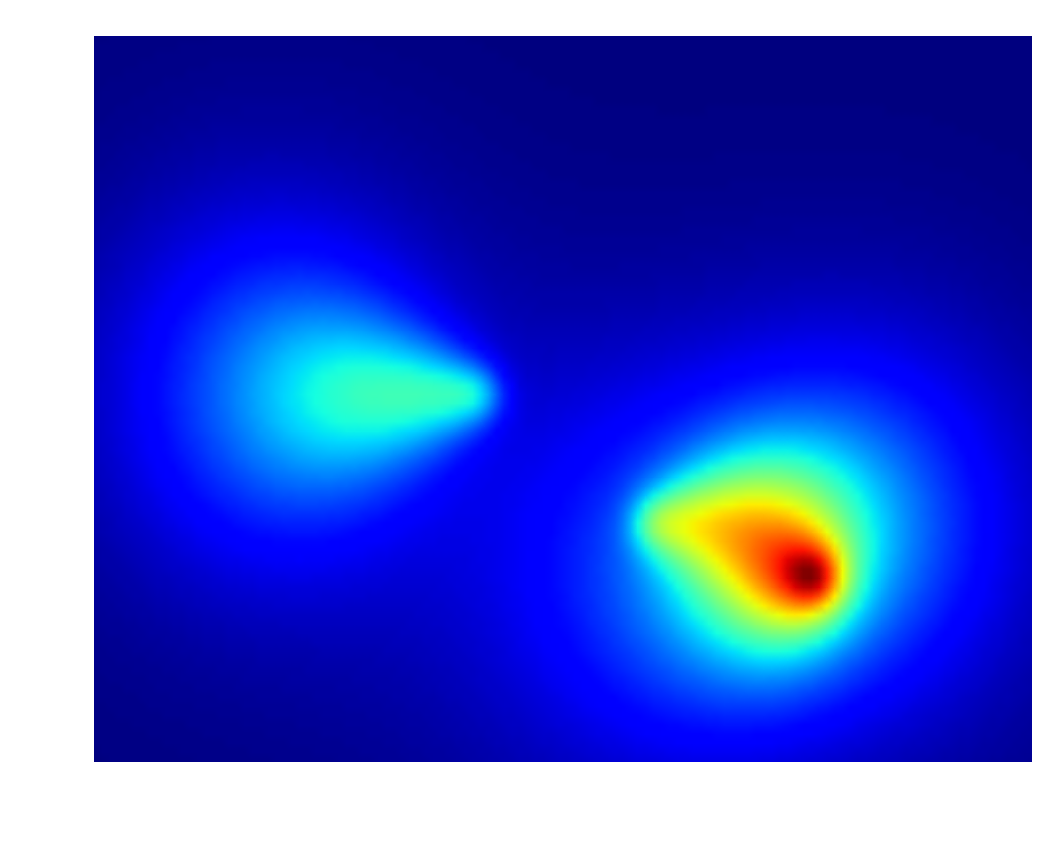
\includegraphics[width=0.32\linewidth]{figs/ex_agent_6}
    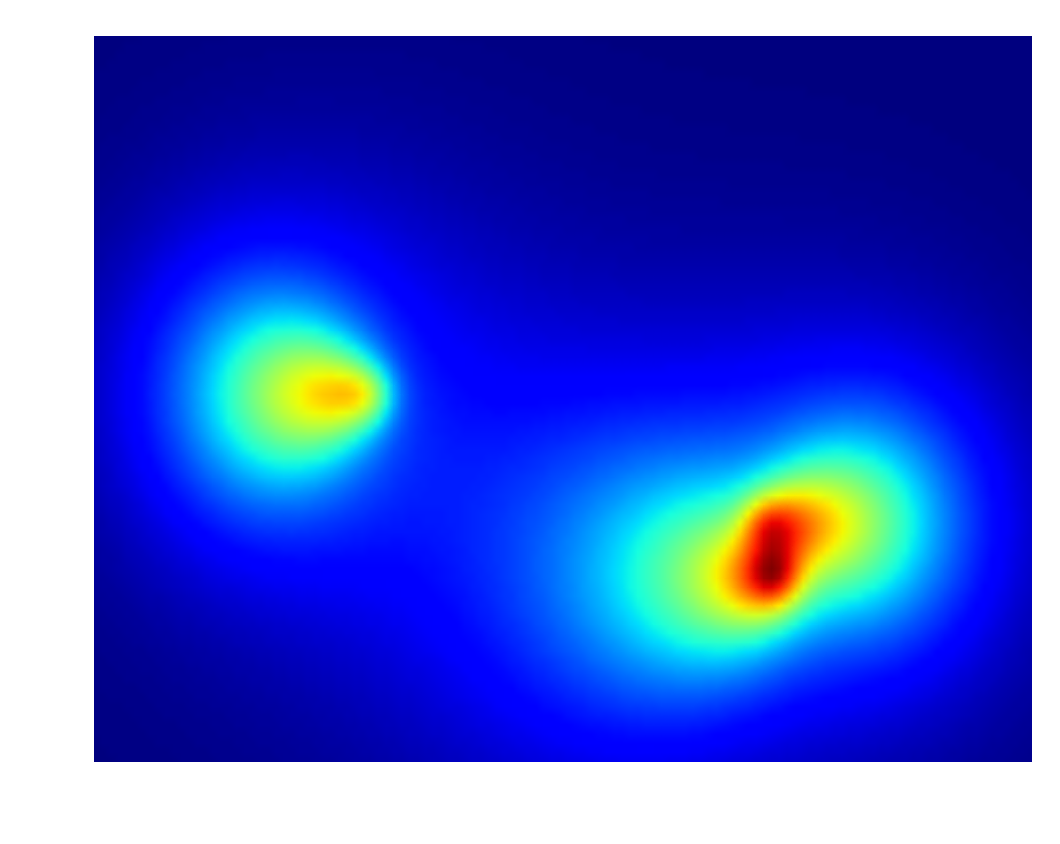
\includegraphics[width=0.32\linewidth]{figs/ex_agent_7}
    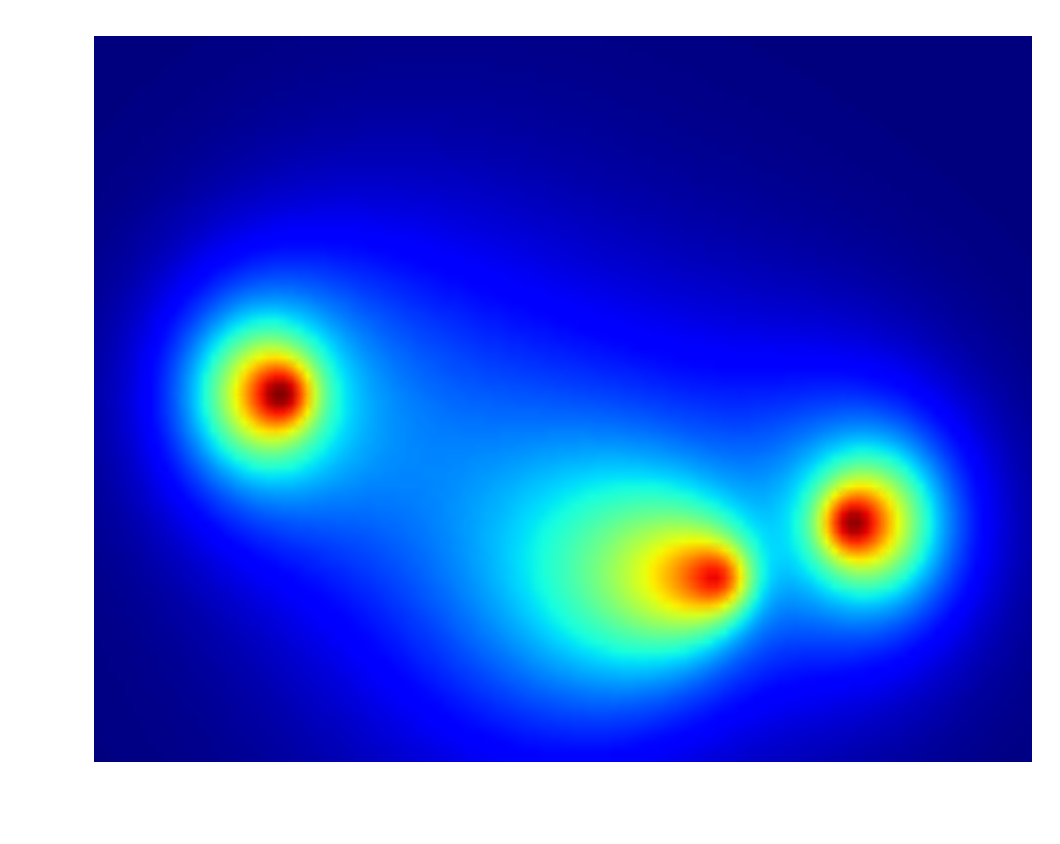
\includegraphics[width=0.32\linewidth]{figs/ex_agent_8}

    \caption{A sequence of images showing the progression of the cost
    distribution for the set of dynamic obstacles over time used for the search
tree shown in Fig.~\ref{fig:tree}. The sequence progresses from left to right,
up to down.}

    \label{fig:ex_agents}
\end{figure}


% % Given a parent dictionary, this returns the backtracked path
% \begin{algorithm}[ht]
%     \caption{$\Function{BacktrackPath}(p, g, t, \mathcal{P})$}
%     % \algorithmicrequire{}
%     % \\\algorithmicensure{}
%     \label{algo:backtrack}
%     \begin{algorithmic}[1]
%         \setcounter{ALC@line}{0}
%         \vspace*{1mm}
%         \STATE $(q, t') \leftarrow (g, t)$
%         \STATE $S \leftarrow \Function{Stack}()$
%         \WHILE {$\mathcal{P}_{(q, t')} \neq (p, 0)$}
%             \STATE $S \leftarrow \Function{Push}(S, (q, t'))$
%             \STATE $(q, t') \leftarrow \mathcal{P}_{(q, t')}$
%         \ENDWHILE
%         \STATE $S \leftarrow \Function{Push}(S, (p, 0))$
%         \RETURN $S$
%     \end{algorithmic}
% \end{algorithm}

\subsubsection{Completeness}

It is important to prove certain properties about the completeness of the
$\Acronym{tBestFS}$ algorithm in order to guarantee that the algorithm will
always return a path in a finite amount of time. For the completeness proof it
is first important to prove properties about the bounds of the two functions
that comprise the total cost function for an edge. The proof for completeness
rests on the fact that the added penalty of returning to a node will be
monotonically increasing as the number of times the node has been visited
increases and that the cost of an edge is strictly finite for all acceptable
parameters. The proof uses these properties to show that in a finite amount of
time, it will be more favourable to expand towards the goal node than to stay
in the same location.

\begin{lemma}

    \label{theorem:increasing}

    The added penalty of returning to a node in the probabilistic roadmap is
    monotonically increasing.

\end{lemma}

\begin{proof}

    Since the added penalty for returning to a node increases by one each time
    the node is visited, as the number of times it has been revisited increases
    to infinity, so does the added penalty.

\end{proof}

\begin{corollary}

    The total cost, $TC$, is a monotonically increasing function.

\end{corollary}

The second property of the functions that make up the edge cost is shown in
Lemma~\ref{theorem:capped} which describes that the cost function, $C$ will
always have a value less than infinity for all permissible parameters.

\begin{lemma}

    \label{theorem:capped}

    The cost for any $(m, n) \in E$ for a time interval $[t, t']$ such that $t'
    - t < \infty$ is strictly less than infinity and $0 < t < t'$.

\end{lemma}

\begin{proof}

    The function, $C$, can only increase to infinity if the two nodes on the
    edge are an infinite distance apart or if the cost distribution in
    Eq.~\ref{eq:singleprob}, $P$, increases towards infinity. For the former,
    two nodes cannot be an infinite distance apart because the connection
    distance, $d$, is set to be strictly less than infinity and because the
    $\forall i, j \in V : ||i - j|| \leq \sqrt{w^2 + h^2}$ where $0 < w <
    \infty$ and $0 < h < \infty$ are the width and height of the scene
    respectively. Therefore $C$ cannot tend to infinity because of the distance
    between nodes since no two nodes are an infinite distance away. For the
    latter, $P$ can only tend to infinity if the normal distribution,
    $\mathcal{N}$ reaches infinity. This is only possible if the variance
    approaches 0. However the variance cannot reach $0$ in this case because
    the constant $\beta$ is always greater than zero. Therefore it is
    impossible for the cost along an edge, $C$, to tend towards infinity.

\end{proof}

Using Lemmas~\ref{theorem:increasing} and~\ref{theorem:capped}, a proof can be
constructed for Theorem~\ref{theorem:completeness} which states that
$\Acronym{tBestFS}$ is complete and will always return a path.

\begin{theorem}

    \label{theorem:completeness}

    $\Acronym{tBestFS}$ will always return a path in a finite amount of time.

\end{theorem}

\begin{proof}

    First, it is important for the proof to note that the penalty for returning
    to a previously visited location increases monotonically to infinity as the
    number of visits for a particular node approaches infinity. Also, the cost
    function, $C$, is bounded strictly below infinity for all possible
    parameters. Now assume the pathological case where $\forall (m, n)
    \in E, \forall i \in \Function{Neighbours}(g) : C(i, g, t, t', A) > C(m, n,
    t, t', A)$ for all time intervals $[t, t']$ and where $g$ is the goal node
    in the probabilistic roadmap. This means that the cost to reach the goal
    will be larger than any edge cost at any time in the graph.  Therefore,
    without the added penalty for returning to a previously visited location,
    the goal will never be popped out of the priority queue for expansion.
    However, since there is a penalty for returning to the same geometrical
    location, as the algorithm progresses, $\forall (m, n)
    \in E, \forall i \in \Function{Neighbours}(g) : TC(i, g, t, t', A, D) <
    TC(m, n, t, t', A, D)$ because each node in the probabilistic roadmap
    except the goal node would have been expanded one or more times, thus
    increasing the added penalty. Since the goal node has not been expanded,
    its total cost would only be the value for $C$ and since $C$ is bounded
    below infinity and the added penalty increases monotonically towards
    infinity, all edges to the goal node would have a lower cost than any edge
    to any other node and thus the goal would be expanded. If the goal is
    expanded, a path to the goal would be returned. The path is returned in a
    finite amount of time because the number of nodes in the graph is finite.

\end{proof}

\subsection{Replanning}

In order to generate safe paths in uncertain, stochastic environments, the
planner is not able to simply provide an \emph{a priori} plan from the
$\Acronym{tBestFS}$ algorithm. It is necessary for the planner to generate new
paths from the current configuration of the robot as it progresses through the
environment if the actual trajectory of a dynamic obstacle deviates too much
from its predicted trajectory. This planning occurs in real-time during the
execution of the path in the environment. This framework for regenerating paths
is called \emph{replanning}. Replanning for this work occurs once the model of
movement for a given dynamic obstacle can no longer predict within an
acceptable error the actual position of the dynamic obstacle. When replanning,
the same probabilistic roadmap is used and the connectivity of the environment
is not resampled.

Replanning works by first generating a preliminary path through the environment
using the $\Acronym{tBestFS}$ algorithm. The robot will then follow this path
by moving at its prescribed constant speed, $s$, in a straight line from node
to node in the path. Once it reaches a node, $i$ at time $t$ in the path, the
robot checks whether the actual locations of the obstacles either sensed by the
robot or by an external system differ more than an acceptable amount, $\delta$,
from the predicted locations of the dynamic obstacles at time $t$ i.e.

$$\bigvee_{a \in A} ||\tilde{\zeta_a}(t) - \zeta_a(t)|| > \delta$$

Where $A$ is the set of dynamic obstacles. If this proposition is true, there
is substantial deviation in the obstacle positions, the planner will update the
value of the dynamic variables, $T$ and $\xi$ for the obstacles which are used
for predicting their trajectories to $t$ and $\tilde{\zeta_a}(t)$ respectively.
These variables are part of the 5-tuple defining the dynamic obstacles which is
described in Sec.~\ref{sec:def}. Once these variables are updated, the graph is
searched using the $\Acronym{tBestFS}$ algorithm starting from the current
position of the robot, $i$ with a starting time of $t$. It is also important to
note that the same dictionary used for storing how many times a node has been
visited when researching the graph. The actual path of the robot is a union of
the past locations of the robot based on the partial paths generated whilst
traversing the environment. Algo.~\ref{algo:path} describes the processes of
replanning due to the deviations in the obstacle locations and is the main
entry point for the Dodger algorithm.

% Main algorithm to get the path
\begin{algorithm}[ht]
    \caption{$\Function{Dodger}(n, d, w, h, \delta, p, g, O, A, R)$}
    \algorithmicrequire{
        \\$n$: Maximum number of samples for the roadmap
        \\$d$: Maximum distance between neighbouring nodes in the roadmap
        \\$w$: Width of the scene
        \\$h$: Height of the scene
        \\$\delta$: Minimum obstacle deviation for replanning
        \\$p$: Starting point of the robot
        \\$g$: Goal point for the robot
        \\$O$: Set of static obstacles
        \\$A$: Set of dynamic obstacles
        \\$R$: Goal radius
    }
    \\\algorithmicensure{
        \\A temporal path from the initial configuration of the robot
        to the goal configuration with replanning.
    }

    \label{algo:path}
    \begin{algorithmic}[1]
        \setcounter{ALC@line}{0}
        \STATE $(V, E) \leftarrow \Function{Roadmap}(n, d, w, h, O)$
        \STATE $\Pi \leftarrow \emptyset$
        \STATE $q \leftarrow p$
        \STATE $t \leftarrow 0$
        \WHILE {$||\Function{Back}(\Pi) - g||_2 > R$}
            \STATE $\pi \leftarrow \Function{SearchGraph}(V, E, R, A, q, g, t)$
            \FORALL {$(i, t') \in \pi$}
                \STATE $\Pi \leftarrow \Pi \cup \{i\}$
                \FORALL {$a \in A$}
                    \STATE $\Function{Step}(a)$
                \ENDFOR
                \IF {$\bigvee_{a \in A} ||\tilde{\zeta_a}(t') -
                    \zeta_a(t')|| > \delta$}
                    \FORALL {$a \in A$}
                        \STATE $T_a \leftarrow t'$
                        \STATE $\xi_a \leftarrow \tilde{\zeta_a}(t')$
                    \ENDFOR
                    \STATE $q \leftarrow i$
                    \STATE $t \leftarrow t'$
                    \STATE $\textbf{break}$
                \ENDIF
            \ENDFOR
        \ENDWHILE
        \RETURN $\Pi$
    \end{algorithmic}
\end{algorithm}

Replanning is necessary because it allows the planner to redirect the robot to
new, safer paths as the environment changes. This is important because the
initial path generated by the $\Acronym{tBestFS}$ algorithm uses the predicted
motion of the obstacles and assumes they will stay on this predicted trajectory
for the execution of the path. The $\Acronym{tBestFS}$ is able to account for
some uncertainty in the motion of the obstacles as described by the cost
distribution in Sec.~\ref{sec:cost} but this distribution is not able to fully
account for path divergences. By updating the information for the dynamic
obstacles and re-searching the probabilistic roadmap using $\Acronym{tBestFS}$,
safer overall paths can be generated. It is possible to regulate the number of
times the planner will need to replan and thus the safety of the plan by
adjusting the value for $\delta$. The larger the value for $\delta$, the more
the obstacles will need to diverge from the prescribed trajectories in order
for the planner to initiate the replanning sequence and vice-versa.

% \subsubsection{Completeness}
%
% \begin{theorem}
%
%     The robot will always reach the goal in a finite amount of time given the
%     proposed replanning scheme outlined in Algo.~\ref{algo:path} for $\delta >
%     0$.
%
% \end{theorem}
%
% \begin{proof}
%
%
%
% \end{proof}

\subsection{Discussion}

\label{sec:plannerdiscussion}

The final algorithm developed is able to generate low cost paths through the
environment by using the available information about the obstacles' motion. The
planner is able to do this by searching through space-time over a two
dimensional graph using the $\Acronym{tBestFS}$ algorithm which uses the cost
distribution described in Sec.~\ref{sec:cost} to weight the edges of the search
tree. The algorithm is also able to adapt and create new plans through the
environment when its' prediction of the obstacles' motion is no longer able to
accurately determine where the obstacles are going to be in future. This
replanning stage of the algorithm allows it to be used in real-time in
stochastic dynamic environments. This mimics the reactive behaviour of
potential fields, with the added benefit of provable completeness and not being
a solely reactive planner. Likewise, the replanning ability allows the
information given to the planner about the motion of the obstacles not to be
perfect. Even if the equations of motion that the motion prediction system
provides in no way describe the actual motion of the obstacles, the algorithm
will simply replan at every time step and instead of using the cost
distributions to determine paths through the environment, the planner will
simply move to the next best node in the probabilistic roadmap. This means that
the algorithm is able to continuously plan through stochastic dynamic
environments utilizing the available information to move the robot to the goal.

\section{Experimental Setup}

\label{chapter:experimentalsetup}

\subsection{Design}

In order to quantify the performance of the developed planner and to judge how
well it performs, experiments needed to be run that can determine the degree of
safety present in the generated paths and how long it takes to generate these
paths. To gather this data, three different scenes were created with differing
number dynamic obstacles with different trajectories. The independent
variables, or parameters, for each scene consisted of the amount of noise,
$\epsilon$ for the dynamic obstacles and the speed of the robot, $s$. For the
experiments, a given value of $\epsilon$ is the same for all of the dynamic
obstacles in the scene. The amount of noise ranges from $0.002$ to $0.01$ with
an increment of $0.002$ and the speed ranges from $1.0$ to $4.5$ meters per
second with an increment of $0.5$ meters per second. Due to the stochasticity
of the planner and the dynamic obstacles, each set of parameters for each scene
was run 20 times. The values for each metric recorded is averaged and the
standard deviation for each set of parameters for each scene is presented.

In order to judge how the developed planner compares to a standard algorithm
developed to plan in stochastic dynamic environments, a slight variant to the
potential fields planner described in Algo.~\ref{algo:pf} was implemented. The
difference is that the implemented potential fields planner used a different
repulsive potential function that is described in Eq.~\ref{eq:betterrep}.

\begin{equation}
    U_{\Var{rep}}(p, t, A) = \max_{a \in A} \,
    \frac{k}{||\tilde{\zeta_a}(t) - g||^2 + \varepsilon}
    \label{eq:betterrep}
\end{equation}

In Eq.~\ref{eq:betterrep}, $k$ is a scaling constant where $k > 0$, and
$\varepsilon$ is constant where $0 < \varepsilon < k$ that ensures that the
function does not exhibit a singularity. This variant in the potential fields
ensures that the planner has no information about the motion of the obstacles
and can thus be used to compare how this information can benefit a planner.
Also, since this planner is not sampling based, it can be used to see how a
complete sampling based planner can be more or less effective. The results from
this experimental setup are described in Ch.~\ref{chapter:results}.

\subsection{Metrics}

To quantify the performance of the planners, four metrics are used, three to
measure the safety and one for computational time. Along with these metrics,
the standard deviation is collected for each scene and set of parameters in
order to gauge the reliability of the planner under different circumstances.
These metrics are described in the sections below.

\subsubsection{Safety}

In order to quantify the safety of a given path $\Pi$, three metrics were
devised. These metrics need to be used together to measure the safety of a path
and each represent a component of what it means for a path to be "safe". The
first metric is the most straightforward and what is probably the first metric
to come to mind, the minimum distance to any dynamic obstacle at any given
time. This metric represents for a given path, what was the closest the robot
came to coming into contact with a dynamic obstacle. Since collisions are more
likely to occur as the robot approaches an obstacle due to the uncertainty in
its motion, this metric serves to provide a simple way of quantifying the
safety without having to account for the motion of the obstacles. This metric
is defined formally in Eq.~\ref{eq:md_metric}.

\begin{equation}
    \Var{MinDist}(\Pi, A) = \min_{t \in \mathcal{T}} \, \min_{a \in A} \,
    ||\zeta_a(t) - \Pi(t)||
    \label{eq:md_metric}
\end{equation}

In Eq.~\ref{eq:md_metric}, $\Pi$ is the path of the robot, $\mathcal{T}$ is the
time interval for the path, and $A$ is the set of dynamic obstacles in the
scene. Since this metric does not account for the motion of obstacles, it
cannot be used as the sole quantification of safety. For example, if the robot
moved near a dynamic obstacle, but was moving in the opposite direction of the
obstacle, the path taken by the robot would still be safe, because there would
be a smaller chance of the robot actually coming into contact with the
obstacle. The robot could have a smaller cost over its path even if it moved
near an obstacle than a robot that was farther away from an obstacle but moved
directly into its trajectory.

Another metric used to compute the safety of a path is the maximum cost
incurred by the robot along the path. This is what the planner described in
Sec.~\ref{sec:design_planner} is trying to minimize. This metric describes how
risky a certain path is by determining the likelihood that the robot's path
would intersect with the trajectory of a dynamic obstacle. A formal definition
of this metric is shown in Eq.~\ref{eq:cost_metric}.

\begin{equation}
    \Var{MaxCost}(\Pi, A) = \max_{t \in \mathcal{T}} \, P(\Pi(t), A)
    \label{eq:cost_metric}
\end{equation}

Since the potential field planner implementation that is used to compare with
the planner created in this work does not utilize the information given about
the cost distribution associated with dynamic obstacles, this metric also
indicates how access to this information can contribute to generating safer
paths through dynamic environments. Since this metric is used to measure the
safety of both the potential fields planner and the developed planner, this
metric can be used to quantify how information about the motion of dynamic
obstacles can either improve or have no effect on the generated paths.

The last metric used to measure the safety of a generated path is the average
cost associated with the robot along the path as determined by the cost
distribution. This metric does not provide the same indication of safety as in
Eq.~\ref{eq:cost_metric} because the overall safety of a path is not just the
average safeness along the path.  For instance if the majority of a path taken
by a robot has a relatively low cost, but then the robot comes into a collision
with an obstacle along the path, this path cannot be labelled as safe.
However, this metric combined with the metrics described in
Eq.~\ref{eq:cost_metric} and Eq.~\ref{eq:md_metric} can be used to gauge the
level of safety for a given path. This last metric is described formally in
Eq.~\ref{eq:avg_cost_metric}.

\begin{equation}
    \Var{AvgCost}(\Pi, A) = \frac{1}{\max \mathcal{T}} \cdot
    \int_{\mathcal{T}} P(\Pi(t), A) \, \mathrm{d}t
    \label{eq:avg_cost_metric}
\end{equation}

Since experiments were conducted with a given set of parameters multiple times
due to the stochasticity of the dynamic obstacles and the developed planner,
each of the metrics were gathered for each individual run. The data gathered
for each of these metrics was then averaged and the standard deviation of the
dataset was determined. As such, it is the averages and standard deviations of
these metrics that are used to quantify the safety of a generated path.

\subsubsection{Computational Time}

In order to determine the feasibility of the paths generated by both planners,
the amount of computational time needed for each planner was collected.
Collecting this data can indicate how well the developed planner can perform in
a real-time scenario. Since the time it takes to compute a path with
replanning, the computational time also represents how long it would take for
the robot to execute the path because it is replanning in real-time.

\subsubsection{Variance}

For each set of parameters, the experiments were conducted multiple times due
to the stochasticity of the dynamic obstacles and the planner. The standard
deviation for each metric and each set of parameters were recorded and used to
indicate how the noise injected into the trajectories of the dynamic obstacles
and the speed of the planner affect the variance in the results. This metric
provides an indication of how consistent the planners will be for different
sets of parameters and can contribute to judging how well each planner will
work in a real world scenario over time.

\subsection{Scenes}

Three different scenes were used for testing the algorithms developed. These
scenes contain oscillating dynamic obstacles with different configurations and
do not contain any static obstacles. No static obstacles were included in the
scenes because the ability to navigate around static obstacles is not the
objective of this project and it is assumed that if the planner is able to
generate paths through dynamic scenes, that they would be able to do so for
static scenes. The images on the following pages depict how the dynamic
obstacles progress over time for each scene. The dynamic obstacles are depicted
as mobile ground robots, and no noise is added to their trajectories for these
examples.

\begin{figure}

    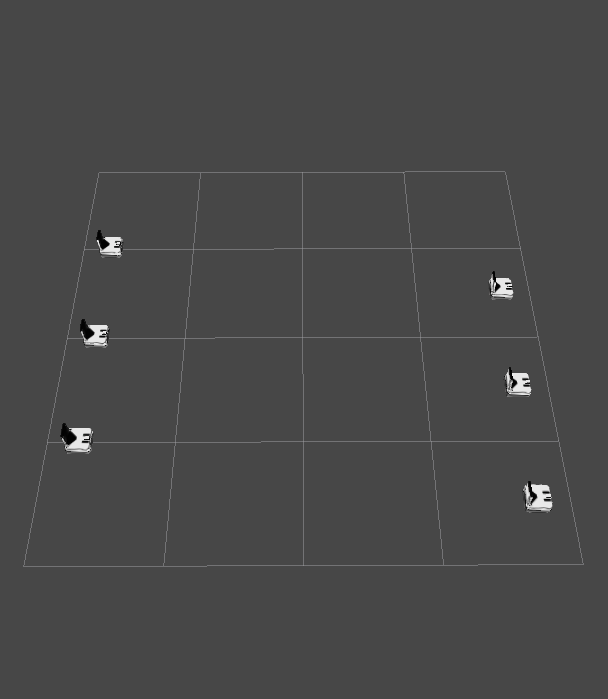
\includegraphics[width=0.24\linewidth]{figs/scene_0_0}
    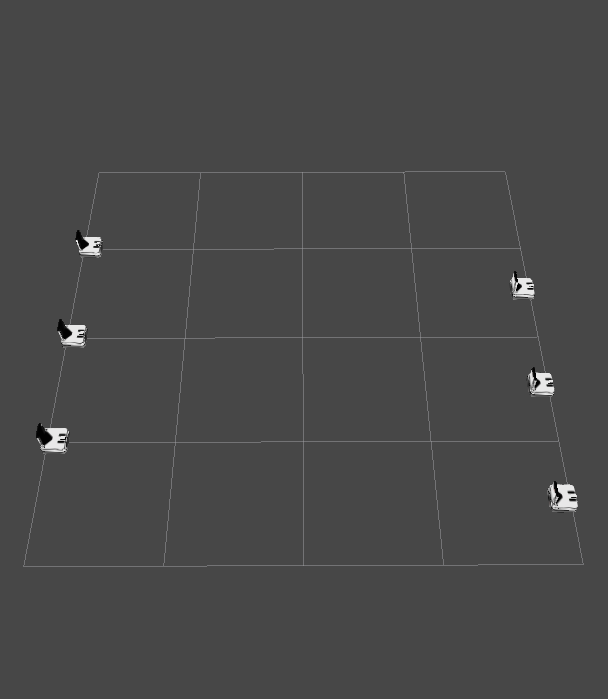
\includegraphics[width=0.24\linewidth]{figs/scene_0_1}
    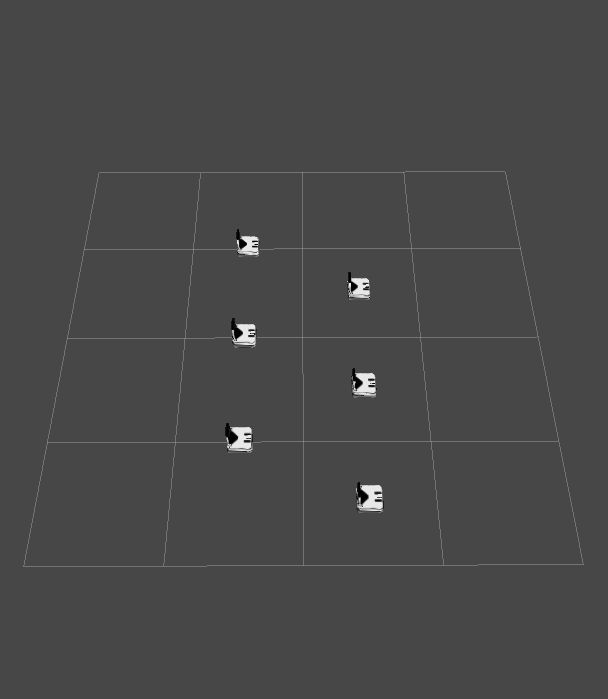
\includegraphics[width=0.24\linewidth]{figs/scene_0_2}
    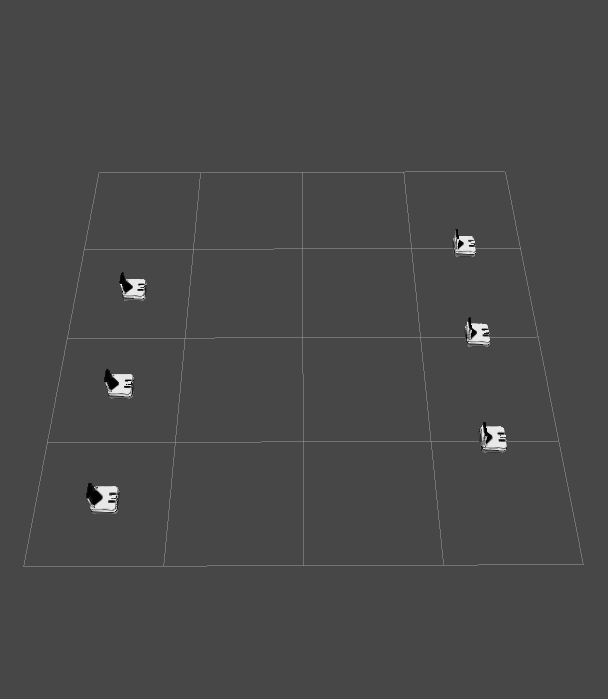
\includegraphics[width=0.24\linewidth]{figs/scene_0_3} \\
    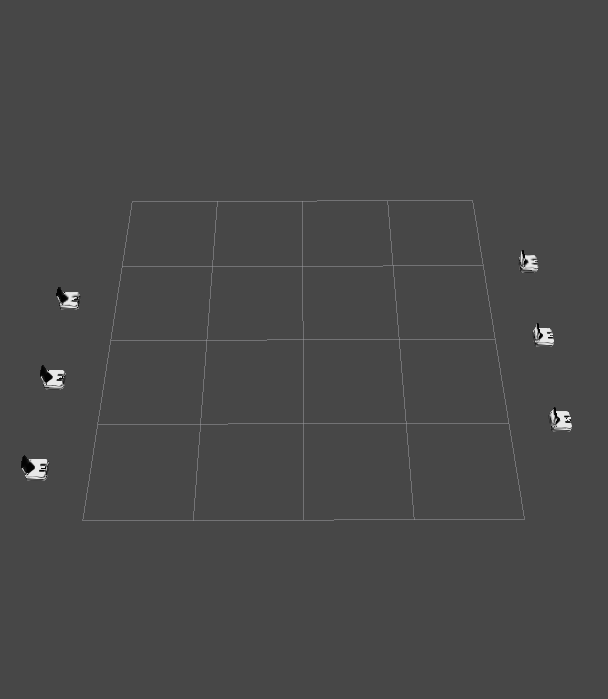
\includegraphics[width=0.24\linewidth]{figs/scene_0_4}
    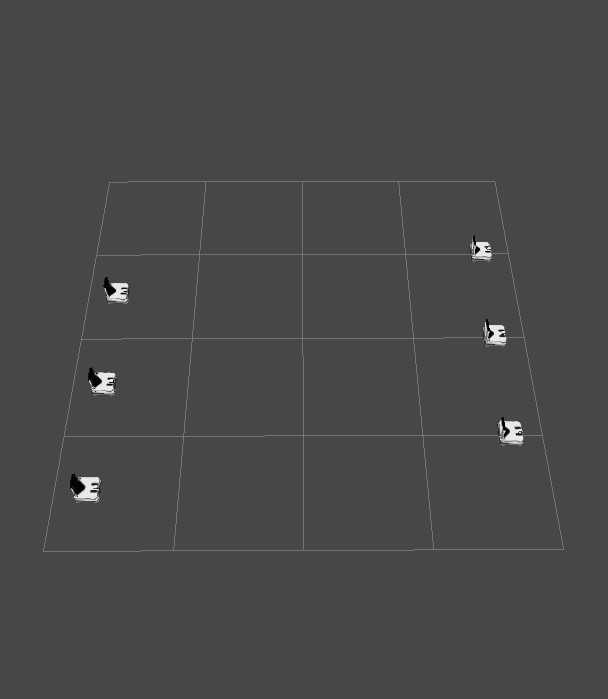
\includegraphics[width=0.24\linewidth]{figs/scene_0_5}
    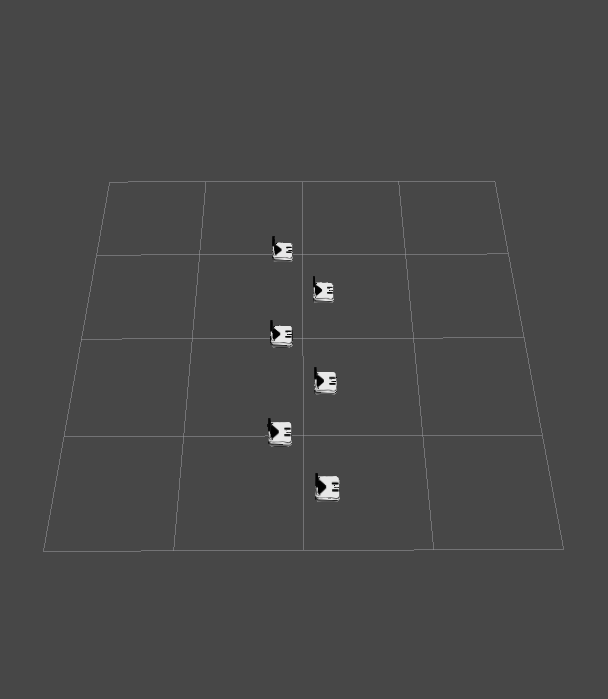
\includegraphics[width=0.24\linewidth]{figs/scene_0_6}
    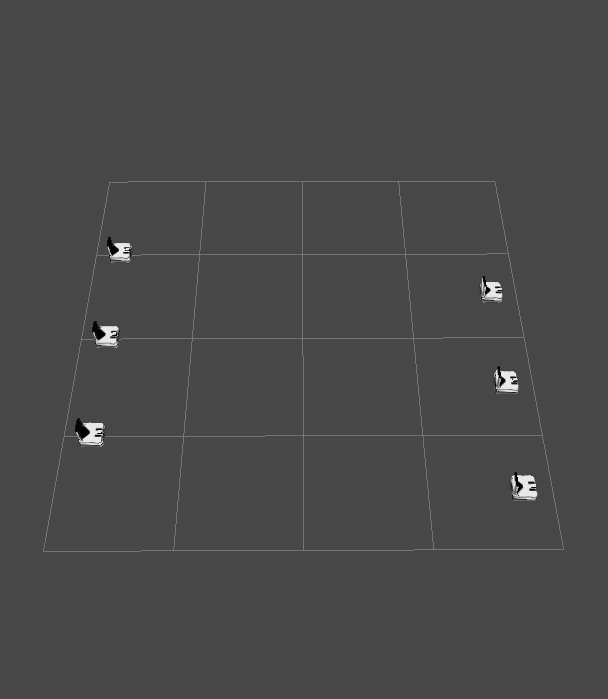
\includegraphics[width=0.24\linewidth]{figs/scene_0_7} \\
    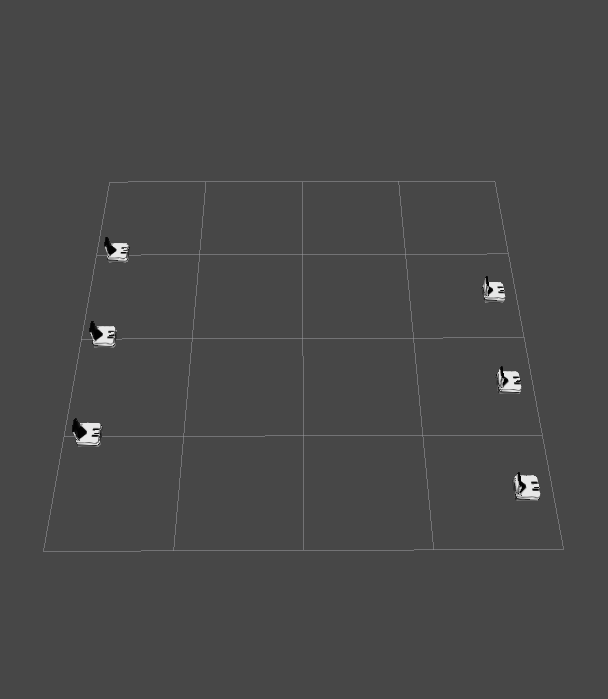
\includegraphics[width=0.24\linewidth]{figs/scene_0_8}
    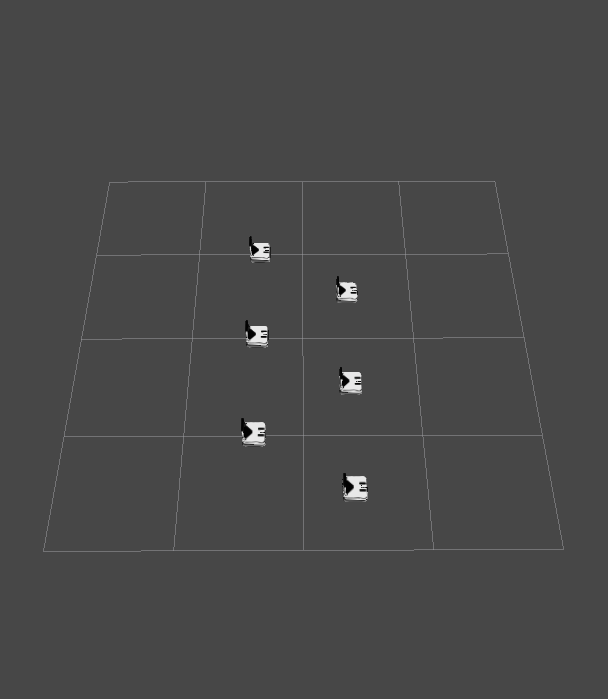
\includegraphics[width=0.24\linewidth]{figs/scene_0_9}
    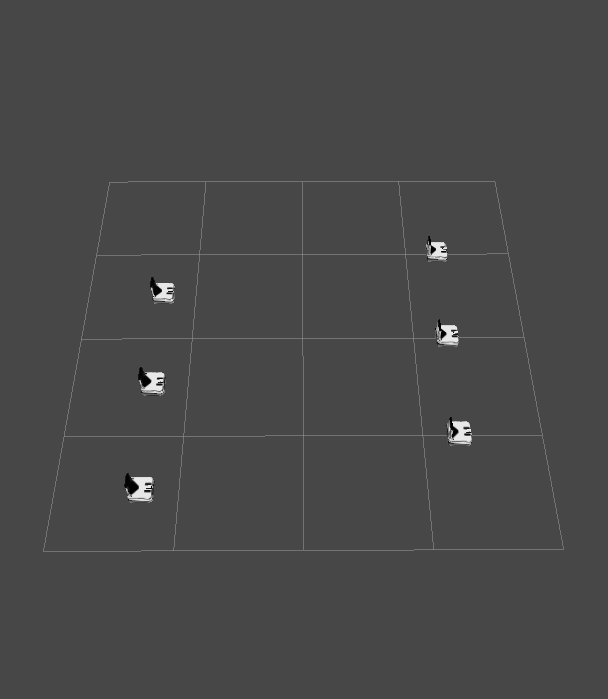
\includegraphics[width=0.24\linewidth]{figs/scene_0_10}
    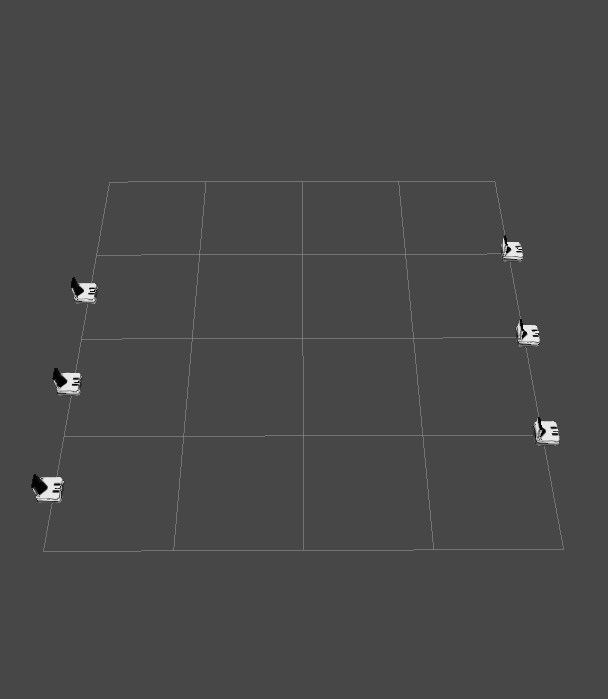
\includegraphics[width=0.24\linewidth]{figs/scene_0_11} \\
    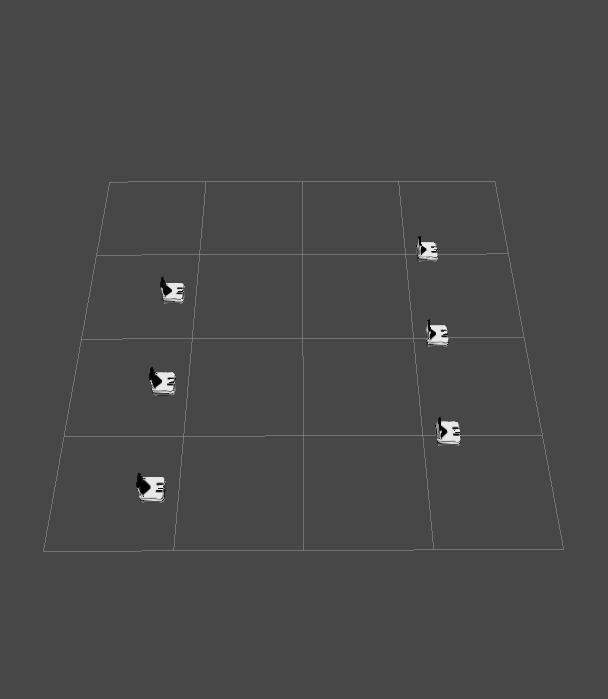
\includegraphics[width=0.24\linewidth]{figs/scene_0_12}
    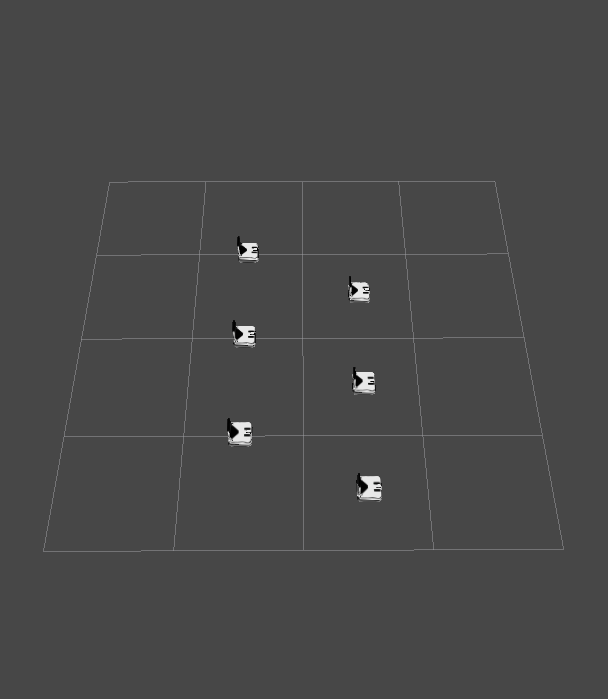
\includegraphics[width=0.24\linewidth]{figs/scene_0_13}
    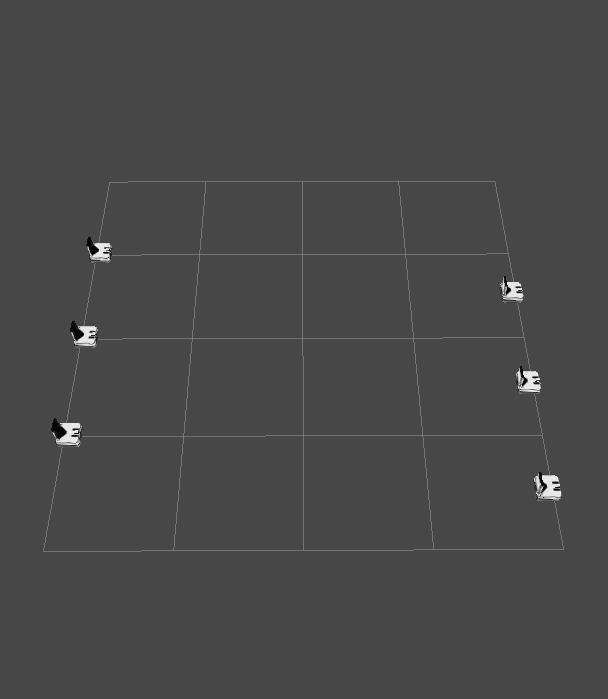
\includegraphics[width=0.24\linewidth]{figs/scene_0_14}
    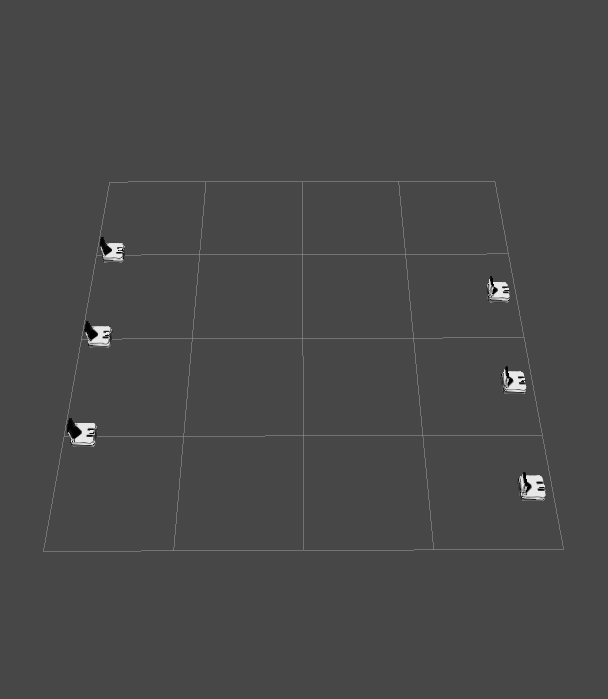
\includegraphics[width=0.24\linewidth]{figs/scene_0_15}

    \caption{A depiction of how the dynamic obstacles progress over time for
    Scene 1. No noise is added to their trajectories in order to display the
pure velocity function used for their motion. The sequences progresses from
left to right, top to bottom.}

    \label{fig:scene_0}

\end{figure}

\begin{figure}

    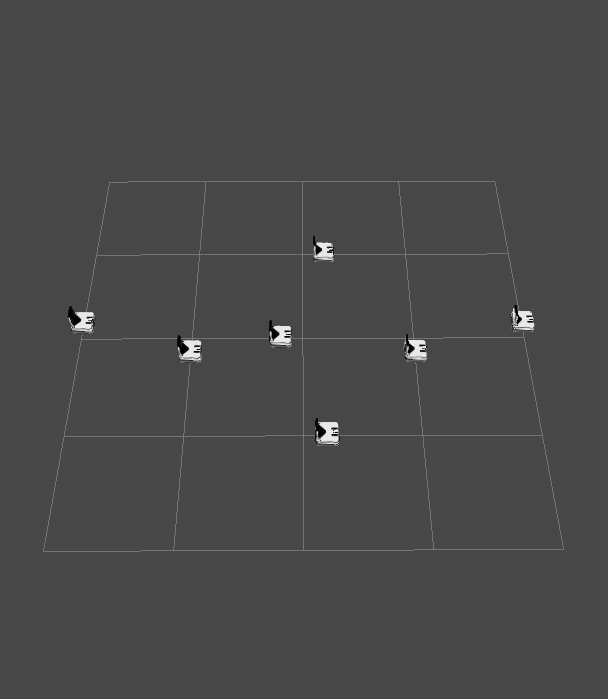
\includegraphics[width=0.24\linewidth]{figs/scene_1_0}
    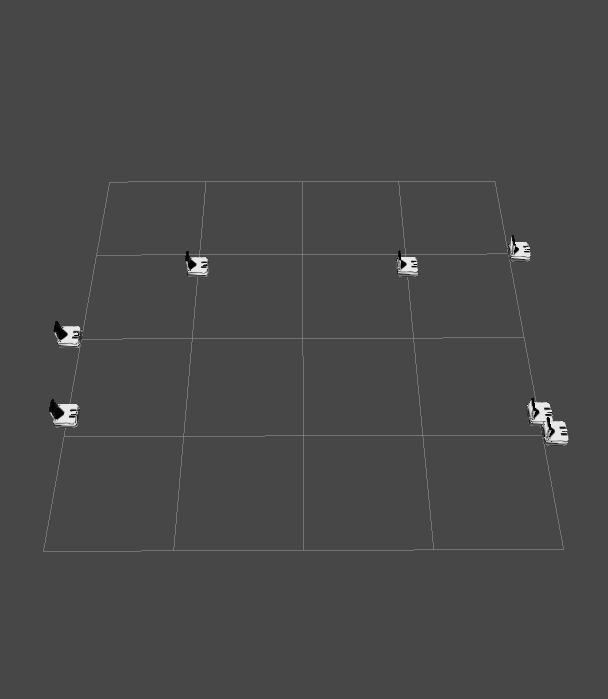
\includegraphics[width=0.24\linewidth]{figs/scene_1_1}
    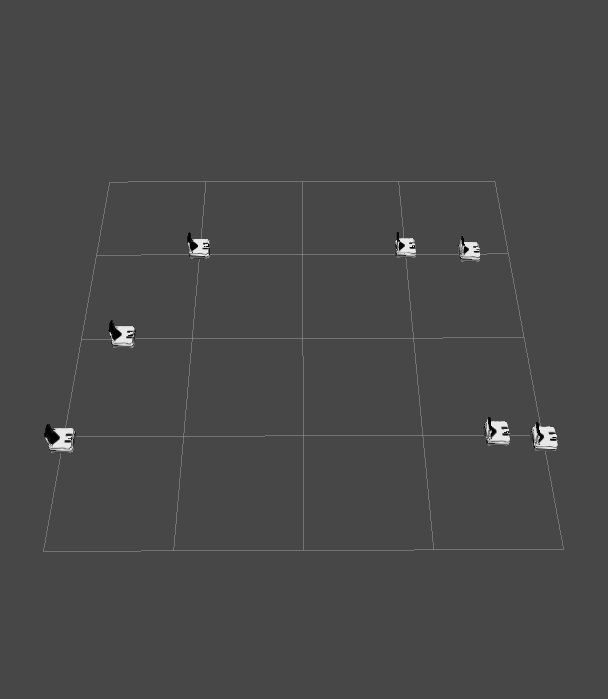
\includegraphics[width=0.24\linewidth]{figs/scene_1_2}
    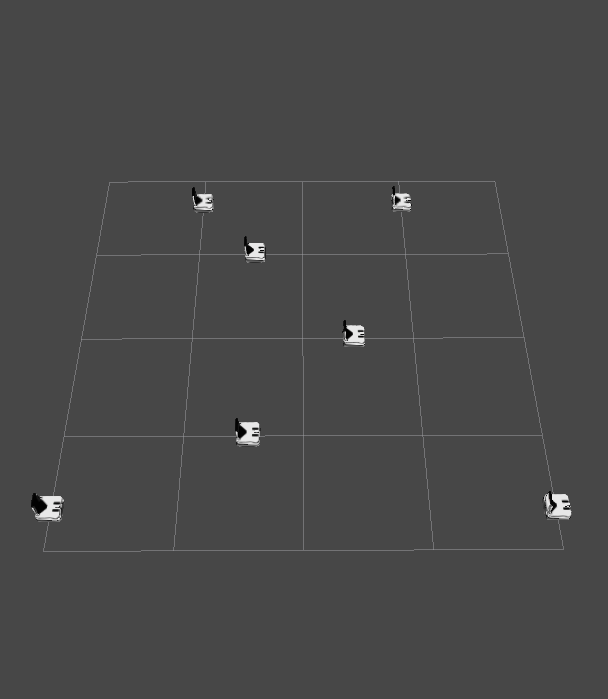
\includegraphics[width=0.24\linewidth]{figs/scene_1_3} \\
    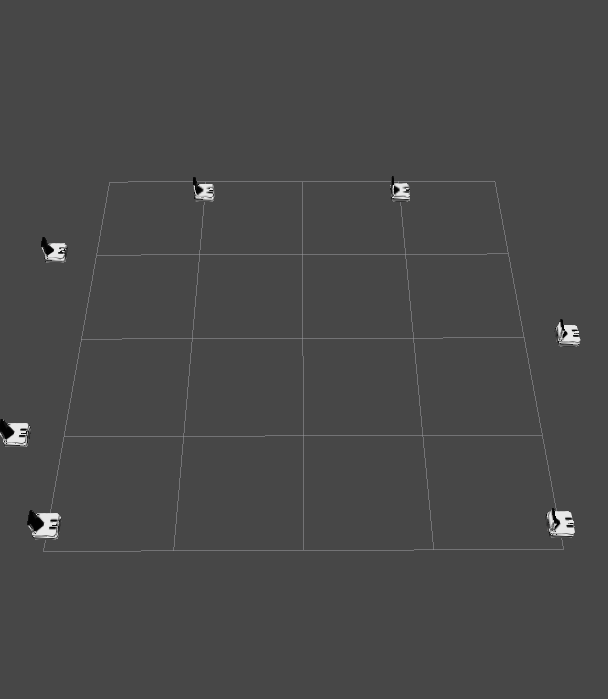
\includegraphics[width=0.24\linewidth]{figs/scene_1_4}
    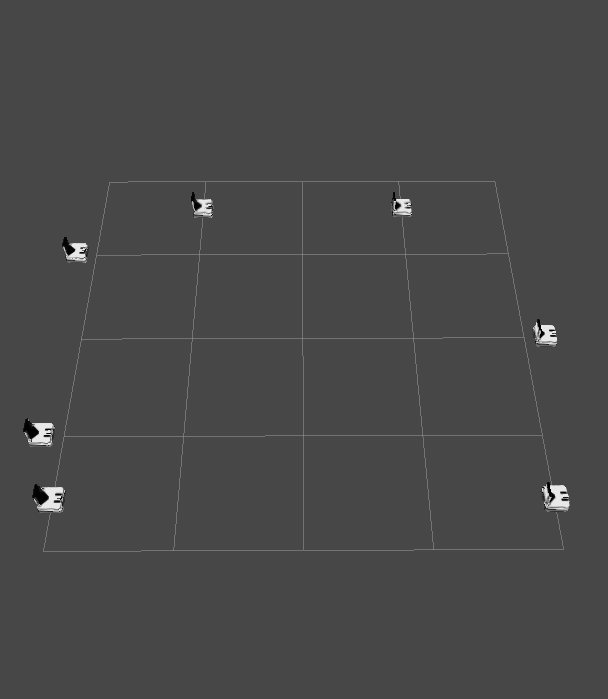
\includegraphics[width=0.24\linewidth]{figs/scene_1_5}
    \includegraphics[width=0.24\linewidth]{figs/scene_1_6}
    \includegraphics[width=0.24\linewidth]{figs/scene_1_7} \\
    \includegraphics[width=0.24\linewidth]{figs/scene_1_8}
    \includegraphics[width=0.24\linewidth]{figs/scene_1_9}
    \includegraphics[width=0.24\linewidth]{figs/scene_1_10}
    \includegraphics[width=0.24\linewidth]{figs/scene_1_11} \\
    \includegraphics[width=0.24\linewidth]{figs/scene_1_12}
    \includegraphics[width=0.24\linewidth]{figs/scene_1_13}
    \includegraphics[width=0.24\linewidth]{figs/scene_1_14}
    \includegraphics[width=0.24\linewidth]{figs/scene_1_15}

    \caption{A depiction of how the dynamic obstacles progress over time for
    Scene 2. No noise is added to their trajectories in order to display the
pure velocity function used for their motion. The sequences progresses from
left to right, top to bottom.}

    \label{fig:scene_1}

\end{figure}

\begin{figure}

    \includegraphics[width=0.24\linewidth]{figs/scene_2_0}
    \includegraphics[width=0.24\linewidth]{figs/scene_2_1}
    \includegraphics[width=0.24\linewidth]{figs/scene_2_2}
    \includegraphics[width=0.24\linewidth]{figs/scene_2_3} \\
    \includegraphics[width=0.24\linewidth]{figs/scene_2_4}
    \includegraphics[width=0.24\linewidth]{figs/scene_2_5}
    \includegraphics[width=0.24\linewidth]{figs/scene_2_6}
    \includegraphics[width=0.24\linewidth]{figs/scene_2_7} \\
    \includegraphics[width=0.24\linewidth]{figs/scene_2_8}
    \includegraphics[width=0.24\linewidth]{figs/scene_2_9}
    \includegraphics[width=0.24\linewidth]{figs/scene_2_10}
    \includegraphics[width=0.24\linewidth]{figs/scene_2_11} \\
    \includegraphics[width=0.24\linewidth]{figs/scene_2_12}
    \includegraphics[width=0.24\linewidth]{figs/scene_2_13}
    \includegraphics[width=0.24\linewidth]{figs/scene_2_14}
    \includegraphics[width=0.24\linewidth]{figs/scene_2_15}

    \caption{A depiction of how the dynamic obstacles progress over time for
    Scene 3. No noise is added to their trajectories in order to display the
pure velocity function used for their motion. The sequences progresses from
left to right, top to bottom.}

    \label{fig:scene_2}

\end{figure}

\section{Results}

\label{chapter:results}

This chapter presents the results from the experimentation of the algorithm.
The metrics used and the experimental setup is described in
Ch.~\ref{chapter:experimentalsetup}. This chapter will describe the empirical
data gathered for the safety and computational time of the algorithm developed
in Sec.~\ref{sec:design_planner}. This chapter will also compare the proposed
approach with a more standard approach, potential fields, using the empirical
data gathered. For all of the plots presented, the data for the algorithm
developed in this work is shown on the left and the data for the standard
potential fields planner is shown on the right. Also note that this chapter
only surveys the results for Scene 1 because the data was very similar for all
of the scenes. The plots for the other scenes are shown in the appendix.

\subsection{Safety}

Providing an empirical evaluation of the safety of the developed planner is
incredibly important because if it does not provide quantifiable safe paths
through the environment, the main objective was not satisfied. This section
presents the data gathered for the three safety metrics with the experimental
setup described in Ch.~\ref{chapter:experimentalsetup}. The three safety
metrics are the minimum distance at any given time during the execution of the
path to a dynamic obstacle, the maximum cost along the path given by the cost
distribution discussed in Eq.~\ref{eq:cost}, and the average cost along the
path.

Fig.~\ref{fig:plot_min_distance} shows how the mean minimum distance changes as
a function of the set speed of the robot and the amount of noise introduced to
the trajectories of obstacles. The larger the minimum distance, the safer the
path is. From the figure, it is evident that as the speed increases, so does
the mean minimum distance Dodger. The amount of noise injected into the
obstacle trajectories, $\epsilon$, does not seem to have any major effect on
the minimum distance for any speed. For potential fields, as the speed
increases, the increase in the minimum distance is not as drastic and the noise
does not affect the overall safety given this metric. The differences between
these two plots stem from the fact that a potential fields planner is purely
reactive and Dodger generates a path by looking ahead. This means that the
potential fields planner could move the robot through the path of an obstacle
thus decreasing the minimum distance and increasing the possibility of a
collision. Dodger will avoid moving the robot through the trajectory of an
obstacle and thus is more likely to have a larger minimum distance along the
path. For the gathered empirical data shown in
Fig.~\ref{fig:plot_min_distance}, Dodger provided paths with a higher overall
minimum distance than potential fields and as the speed of the robot increased,
the minimum distance for the paths generated by Dodger out performed those
generated by potential fields for this metric.

\begin{figure}[h!]
    \centering
    \includegraphics[width=0.48\linewidth]{figs/planner_mean_min_distance_0}
    \includegraphics[width=0.48\linewidth]{figs/pf_mean_min_distance_0}

    \caption{Plots showing how the minimum distance to any obstacle for a path
        changes as the speed increases for various amounts of obstacle position
        uncertainties.  The horizontal axis represents the speed of the robot
        and the vertical axis represents the minimum distance to obstacles
        along the path. The different lines on each plot represent experiments
    with differing amounts of noise and the error bars represent one standard
deviation. On the left is the graph for Dodger and on the right is the graph
for the potential fields planner.}

    \label{fig:plot_min_distance}
\end{figure}

Fig.~\ref{fig:plot_max_cost} shows how the maximum cost experienced along a
path given by the cost distribution changes as a function of the set speed of
the robot. The smaller the maximum cost, the safer the path. The figures shows
that as the speed increases, the maximum cost experienced by a robot being
planned using Dodger decreased. This is because when the robot is able to move
faster, it can maneuver through areas that only have a low cost for a small
period of time before becoming high cost areas again. Also, as the speed
increased over 2 $m/s$, there was a greater difference between the maximum
costs for paths through experimental configurations with small amounts of noise
and the maximum costs for paths through high noise configurations.  This is due
to the fact that no matter how fast the robot is able to move, the more noise
in a scene, the more the initial path will not represent the actual costs
through the environment and the planner will need to replan. The robot may move
to an area in which it thinks it will be safe, but if the obstacles deviate
from their prescribed trajectories, this area may not be safe any longer and a
new path is needed and therefore the cost for the path a robot is executing
will increase.  The paths generated by the potential fields planner did not
have a similar behaviour as the amount of noise increased, however, the maximum
cost was greater for all speeds than that of the paths generated by Dodger.
This is because the potential fields planner does not take into account the
trajectories of the obstacles when planning and is purely reactive. This plot
shows that having access to information about where obstacles are moving can
decrease the costs of the generated paths which in turn leads to safer
trajectories for the robot.

\begin{figure}[h!]
    \centering
    \includegraphics[width=0.48\linewidth]{figs/planner_mean_max_cost_0}
    \includegraphics[width=0.48\linewidth]{figs/pf_mean_max_cost_0}

    \caption{Plots showing how the maximum cost for a path changes as the
        speed increases for various amounts of obstacle position uncertainties.
        The horizontal axis represents the speed of the robot and the vertical
        axis represents the maximum cost along the path. The different lines on
    each plot represent experiments with differing amounts of noise and the
error bars represent one standard deviation.  On the left is the graph for
Dodger and on the right is the graph for the potential fields planner.}

    \label{fig:plot_max_cost}
\end{figure}

Fig.~\ref{fig:plot_avg_cost} shows how the average cost along a path changes as
the speed of the robot increases for Dodger and the potential fields planner.
These plots are very similar to those in Fig.~\ref{fig:plot_max_cost} however,
there is an increase in the average cost for the potential fields. This is
mostly likely because as the speed of the robot increases, the potential fields
planner is able to move the robot through the path of an obstacle without being
deviated or hit by the obstacle thus increasing the average cost along the
path. Since the planner can move the robot through these areas quickly, instead
of planning around the obstacle, the planner will just move quickly through the
path of the obstacle. From these plots, it is evident that Dodger was able to
generate paths with lower average costs than potential fields and as the speed
of the robot increased, the average costs of the paths for Dodger decreased
whereas the costs for paths generated by potential fields increased.

\begin{figure}[h!]
    \centering
    \includegraphics[width=0.48\linewidth]{figs/planner_mean_avg_cost_0}
    \includegraphics[width=0.48\linewidth]{figs/pf_mean_avg_cost_0}

    \caption{Plots showing how the average cost for a path changes as the
        speed increases for various amounts of obstacle position uncertainties.
        The horizontal axis represents the speed of the robot and the vertical
        axis represents the average cost along the path. The different lines on
    each plot represent experiments with differing amounts of noise and the
error bars represent one standard deviation.  On the left is the graph for
Dodger and on the right is the graph for the potential fields planner.}

    \label{fig:plot_avg_cost}
\end{figure}

\subsubsection{Variance}

Representing the standard deviation as a function of the noise quantifies how
consistent the planner is as the noise for a scene changes.The plots in
Fig.~\ref{fig:plot_std_min_distance} show how the standard deviation for the
minimum distance metrics increases as the noise injected into the obstacle
trajectory increases and the speed changes. The standard deviation for minimum
distance metric increased more rapidly for Dodger than for the potential fields
planner.  This is because there is a stochastic component in the planning for
Dodger, the probabilistic roadmap. For some random generations of the roadmap,
areas around where the obstacles are going to be are more heavily sampled, thus
leading to greater variance in the results for the minimum distance. For the
potential fields planner, there is no random component and is free to sample
along the execution of its path and thus the standard deviation for this metric
is only determined by the stochasticity of the dynamic obstacles and not by the
algorithm.

\begin{figure}[h!]
    \centering
    \includegraphics[width=0.48\linewidth]{figs/planner_std_min_distance_0}
    \includegraphics[width=0.48\linewidth]{figs/pf_std_min_distance_0}

    \caption{Plots showing how the standard deviation for the minimum distance
        along a path changes as the noise injected into the obstacle
        trajectories increases. The horizontal axis represents the amount of
        noise and the vertical axis represents the standard deviation. The
        different lines indicate different speeds that the robot was
    travelling. On the left is the graph for Dodger and on the right is the
graph for the potential fields planner.}

    \label{fig:plot_std_min_distance}
\end{figure}

The plots in Fig.~\ref{fig:plot_std_cost} shows how the average and maximum
costs change as the noise injected into the obstacle trajectories increases.
The average and minimum costs for the paths generated by Dodger increases less
rapidly than those generated by the potential fields planner. This is because
Dodger is actively searching for low cost paths through the environment using
the information about obstacle motion whereas the potential fields planner is
just reacting the change in the potentials leading to the goal. Since the
potential fields planner is not trying to minimize the cost of the generated
path, there will be a larger variance in the average and maximum costs.

\begin{figure}[h!]
    \centering
    \includegraphics[width=0.48\linewidth]{figs/planner_std_max_cost_0}
    \includegraphics[width=0.48\linewidth]{figs/pf_std_max_cost_0} \\
    \includegraphics[width=0.48\linewidth]{figs/planner_std_avg_cost_0}
    \includegraphics[width=0.48\linewidth]{figs/pf_std_avg_cost_0}

    \caption{Plots showing how the standard deviation for the maximum cost and
        average cost along a path changes as the noise injected into the
        obstacle trajectories increases. The horizontal axis represents the
        amount of noise and the vertical axis represents the standard
        deviation. The different lines indicate different speeds that the robot
        was travelling. On the left is the graph for Dodger and on the right is
    the graph for the potential fields planner. The top row is for the maximum
cost and the bottom row is the for the average cost.}

    \label{fig:plot_std_cost}
\end{figure}

\subsection{Computational Time}

Showing how the computational time changes for different sets of parameters is
useful to show how feasible the approach is in practice. For the two planners,
the times it took to compute the paths were collected and are shown in
Fig.~\ref{fig:plot_comp_time}. The potential fields planner is able to find
paths more quickly than Dodger and this is due to its purely reactive
behaviour.  Since the scenes used did not have any local minimas besides the
goal, the potential fields planner is able to quickly find a path to the goal
and as the speed increases, the amount of steps needed for it to search through
the environment decreases thus decreasing the overall computational time.  The
computational time for Dodger also decreased as the speed increased, but the
overall computational time was greater than potential fields. This is because
Dodger uses a much more complex algorithm than potential fields requiring more
computational time. For speeds less than 2.5 $m/s$, the time it takes Dodger to
find a path may be infeasible for some situations.  However, for speeds of 2.5
$m/s$, the computational time decreasing drastically making it feasible to use
for real-time scenarios.  Please note that computational times shown in
Fig.~\ref{fig:plot_comp_time} represent the overall time it takes the planner
to find a path with replanning.  This means that the planner is simultaneously
executing and planning thus meaning that the robot reached the goal in at least
the time presented in the figures.

\begin{figure}[h!]
    \centering
    \includegraphics[width=0.48\linewidth]{figs/planner_mean_times_0}
    \includegraphics[width=0.48\linewidth]{figs/pf_mean_times_0} \\
    \includegraphics[width=0.48\linewidth]{figs/planner_small_mean_times_0}
    \includegraphics[width=0.48\linewidth]{figs/pf_small_mean_times_0}

    \caption{Plots showing how the computational to generate a path changes as
        the speed increases for various amounts of obstacle position
        uncertainties.  The horizontal axis represents the speed of the robot
        and the vertical axis represents the computational time to generate the
        path. The different lines on each plot represent experiments with
        differing amounts of noise and the error bars represent one standard
        deviation.  On the left is the graph for Dodger and on the right is the
    graph for the potential fields planner.}

    \label{fig:plot_comp_time}
\end{figure}

\subsubsection{Variance}

As with the other metrics, seeing how the variance reacts to an increasing
amount of noise is equally as important. Fig.~\ref{fig:plot_std_comp_time}
presents this relationship. The standard deviations for computational times for
Dodger increase more rapidly than for the potential fields planner. This is
because the Dodger had significantly larger computational times than the
potential fields planner and would also have higher standard deviations.
Likewise, the computational time standard deviations for Dodger are caused by
both the randomness of the nodes used to create the probabilistic roadmap and
the level of uncertainty injected into the obstacle trajectories. The standard
deviation for the computational times for the potential fields planner is only
dependent on the amount of noise in the obstacles movements since the algorithm
does not have any random components.

\begin{figure}[h!]
    \centering
    \includegraphics[width=0.48\linewidth]{figs/planner_std_avg_times_0}
    \includegraphics[width=0.48\linewidth]{figs/pf_std_avg_times_0}

    \caption{Plots showing how the standard deviation for the computational
        cost to generate a path changes as the noise injected into the obstacle
        trajectories increases.  The horizontal axis represents the amount of
        noise and the vertical axis represents the standard deviation. The
    different lines indicate different speeds that the robot was travelling. On
the left is the graph for Dodger and on the right is the graph for the
potential fields planner.}

    \label{fig:plot_std_comp_time}
\end{figure}

\subsection{Behaviour}

Figures~\ref{fig:dodger} and~\ref{fig:pf} show how Dodger and the potential
fields planner respectively guide the robot through Scene 1 when the noise
injected into the obstacle trajectories, $\epsilon = 0.004$ and the speed, $s =
1.5 m/s$. The robot is represented by the quadrotor, its path by the blue line,
the obstacles by the mobile ground robots, and the initial and goal
configurations by the red and green quadrotors respectively. Qualitatively, the
paths generated by Dodger look safer than that of those generated by the
potential fields planner.  The potential fields planner even led the robot into
collisions twice in the third and sixth snapshots in Fig.~\ref{fig:pf}. This is
because the obstacles are not within the sensing radius of the robot using
potential fields until they are at their maximum velocity in the center of the
scene and the robot is not able to move out of their way. Dodger generates a
path that automatically moves the robot around the back of the oscillating
obstacles such that it does not cross over their trajectories from side to
side. This reduces the cost associated with the path and significantly reduces
the chance that the robot will collide with an obstacle. Due to the
stochasticity of the obstacles' movements, Dodger needed to replan more than
once when executing the initial path. This occurred right before images three,
four, and six. The path becomes jagged and changes direction quickly. This is
because the original path is no longer safe because of the random movement of
the obstacles.

\begin{figure}[h!]
    \centering
    \includegraphics[width=0.32\linewidth]{figs/dodger_0}
    \includegraphics[width=0.32\linewidth]{figs/dodger_1}
    \includegraphics[width=0.32\linewidth]{figs/dodger_4} \\
    \includegraphics[width=0.32\linewidth]{figs/dodger_6}
    \includegraphics[width=0.32\linewidth]{figs/dodger_9}
    \includegraphics[width=0.32\linewidth]{figs/dodger_12} \\
    \includegraphics[width=0.32\linewidth]{figs/dodger_13}
    \includegraphics[width=0.32\linewidth]{figs/dodger_16}
    \includegraphics[width=0.32\linewidth]{figs/dodger_19}

    \caption{Images showing the progression of the robot, represented by the
    quadrotor, following a path generated by Dodger through Scene 1 from the
initial configuration, represented by the red quadrotor shape, to the goal
configuration, the green quadrotor shape.  The obstacles are represented by the
mobile ground robots and the path of the robot is shown by the blue line. The
sequence of images progress from left to right, up to down.}

    \label{fig:dodger}
\end{figure}

\begin{figure}[h!]
    \centering
    \includegraphics[width=0.32\linewidth]{figs/pf_0}
    \includegraphics[width=0.32\linewidth]{figs/pf_1}
    \includegraphics[width=0.32\linewidth]{figs/pf_3} \\
    \includegraphics[width=0.32\linewidth]{figs/pf_6}
    \includegraphics[width=0.32\linewidth]{figs/pf_9}
    \includegraphics[width=0.32\linewidth]{figs/pf_12} \\
    \includegraphics[width=0.32\linewidth]{figs/pf_13}
    \includegraphics[width=0.32\linewidth]{figs/pf_16}
    \includegraphics[width=0.32\linewidth]{figs/pf_19}

    \caption{Images showing the progression of the robot, represented by the
    quadrotor, following a path generated by the potential fields planner
    through Scene 1 from the initial configuration, represented by the red
    quadrotor shape, to the goal configuration, the green quadrotor shape.  The
    obstacles are represented by the mobile ground robots and the path of the
robot is shown by the blue line. The sequence of images progress from left to
right, up to down.}

    \label{fig:pf}
\end{figure}

\section{Future Work}

There are many possible improvements to this project that could not be
accomplished in the given time frame. This section addresses these future
improvements and how they can impact the performance and robustness of the
project.

\subsection{Pruning the Search Tree}

Currently, the only mechanism used to prune the search tree is the priority of
the nodes being expanded. This allows some nodes in the probabilistic roadmap
not to be expanded thus limiting the overall size of the tree. However, more
complex machine learning techniques could be used such as limiting the density
of the search tree in certain areas and not expanding nodes in a geometric area
that have consistently shown to have higher costs. Pruning the search tree
could have drastic result in reducing the computational time needed to find a
safe path because less nodes would need to be expanded and searched. Another
approach at limiting the size of the search tree could be to use another
heuristic that could provide some information about how close a certain node is
to reaching the goal. This would find paths to the goal more quickly because
the search is more directed. There would have to be some constraints used in
this heuristic, for instance, its influence in the priority of a node in the
queue because the safeness of a path would be sacrificed in return for
decreased computational time. Likewise, decreasing the average degree of a node
in the probabilistic roadmap whilst ensuring that the probabilistic roadmap is
one connected component would limit the size of the search tree and thus the
computational time.  This could be done by using alternative roadmap
construction methods such as connecting the $k$-nearest neighbours instead of
all nodes within a given radius.

\subsection{Variable Speed and Wait Time}

There are two constants in this work, the speed and wait time, which if made
made dynamic would increase the robustness of the algorithm. It is assumed that
the robot will travel at a constant speed at all times unless it is waiting for
a set period of time. However, there may be some reasons for increasing or
decreasing the speed of the robot during runtime. For instance, if the robot
were to also try and save energy, it may not to maintain a high speed, but only
increase its speed when it is needed to avoid coming into contact with
obstacles in order to improve safety and minimize energy usage. Also,
determining dynamically how long the robot should wait at a given location
instead of having a set length of time would increase the robustness of the
approach. By using a constant wait time, it is assumed that that interval is
the best possible amount of time to stay stationary. In reality, in some
situations, the robot will need to wait for longer than others. This is
currently not incorporated into the approach and would be a valuable addition.

\subsection{Increasing Robot Dimensionality}

In the current work, it is assumed that the robot is a two dimensional point in
space. This means that the robot occupies at any given time a certain point in
space and that point in space exclusively. Many robot systems operate in higher
dimensional spaces such as snake robots and unmanned aerial vehicles. Snake
robots operate in the same dimension as the number of links it has. Unmanned
aerial vehicles operate in three dimensional space because they are able to
fly. By incorporating higher dimensional vehicle models into the algorithm,
paths for more classes of robots can be generated and thus makes the approach
more robust.

\subsection{Real World Experiments}

Since this project is concerned with moving a physical robot through an
environment, an important piece of future work would be to conduct experiments
using a physical robot in a real-world scenario. This would mean adapting the
path generated for the robot into a list of control inputs that would account
for the physics of the robot to move it to the goal. Since the project provides
a sequence of spatio-temporal waypoints, a specialized controller can be
created for different mobile robots that could follow the waypoints generated.
It may also be beneficial to utilize the control model for the given robot into
the planning. So instead of the result of the planning algorithm returning a
sequence of waypoints, it could directly return a sequence of control inputs
that could be fed into a robot's controller to move it to the goal. Another
important component of implementing the system on a mobile robot would be the
active prediction of obstacle movements. In this work, it is assumed that there
is an external system being used that can determine where obstacles are going
to move in the future. This system would either have to be implemented or an
existing one used in order for the algorithm to work in real-time. This motion
prediction system could either be its own component in an open loop system
(like those found in warehouses), or the motion prediction could occur directly
on the robot. If it is the latter, novel algorithms are going to need to be
developed that are able to predict the motion of obstacles relatively quickly
due to the limits set by the robot's processing power.

\subsection{More Complex Models of Obstacle Behaviour}

Obstacle behaviour in the current work is very simple. Obstacles are assumed to
move along their prescribed trajectory with a set amount of uncertainty and are
not affected by the actions of the robot or the other obstacles near it. It is
also assumed that the obstacles will only follow one trajectory function and
the current formulation does not account for obstacles with dynamic trajectory
equations. The goal of future work would be to formalize a more complete model
of the way an obstacle moves through the environment by incorporating reactive
behaviour and multiple trajectory equations with associated spatio-temporal
probabilities of switching between them. The reactive behaviour will encompass
how the obstacle will react when other objects, either other obstacles or the
robot being planned, move toward the obstacle or interfere with its trajectory.
Likewise, the obstacles can be assumed to also be autonomous agents with their
own planning algorithm. Accounting for this behaviour will result in a more
comprehensive and realistic model of dynamic obstacles.

\subsection{Multi-robot Coordination}

Another extension to the current algorithms provided in this work would be to
allow them to plan for multiple robots simultaneously. The current
implementation only provides a path through a stochastic dynamic environment
for a single robot. Many applications of robotics need multiple robots to move
through the environment safely and at the same time. These algorithms are
usually called swarming algorithms. By extending the current algorithms to find
the $k$-safest paths through the environment in space-time, paths can be
generated for multiple robots and thus safely plan the movements of a swarm to
its goal.

\section{Evaluation \& Conclusion}

From the results of the experiments shown in Ch.~\ref{chapter:results}, it is
evident that the algorithms proposed in this work are able to generate
quantitatively and qualitatively safer paths than potential fields, a standard
approach at planning through stochastic dynamic environments. As the speed
increased, the paths generated by Dodger had higher minimum distances to
obstacles and lower maximum and average costs along the path. This means that
Dodger could generate paths that stayed farther away from obstacles than
potential fields. Also, since it has information about where the obstacles are
moving, the cost incurred by the robot along the paths generated by Dodger were
lower than those generated by the potential fields planner. The paths did take
longer to compute by Dodger than the potential fields planner, but the times
were reasonable enough to use a real-time scenario. As computers become smaller
and their processing power increases, the computational time needed to generate
a path will decrease. For both planners and all metrics, the standard
deviations increased at roughly the same rate as the noise injected into the
trajectories of the obstacles increased. This is because the variance in the
results are highly dependent on the motions of the obstacles. The more
uncertainty in the obstacle trajectories, the more each planner will have to
adjust its plan to cope.

From the metrics described in Ch.~\ref{chapter:experimentalsetup} Dodger is
able to outperform a standard approach for planning in stochastic dynamic
environments. The algorithms developed are able to leverage the information
available about the motions of obstacles in order to guide a robot along safe,
low cost paths from an initial configuration to a goal configuration. Dodger is
also able to actively generate new paths in real-time to the goal configuration
if it senses that the obstacles have deviated too far from their prescribed
trajectories. This replanning enables the robot to react to the stochasticity
and uncertainty of the environment and maintain a safe trajectory to the goal.
The novel representation of dynamic obstacles and the algorithms used to plan
around them shed light on a new way of path planning that can make use of
available information from the environment to keep the robot and more
importantly, the agents acting in the environment (i.e. humans, cars, other
robots, etc) safe.


\bibliographystyle{IEEEtran}
\bibliography{mp}

\end{document}

